\section{Type models and type graphs}
\label{sec:transformation_framework:type_models_and_type_graphs}

In this section, the proposed framework structure is applied to type models and type graphs. First, the general structure and its requirements are discussed. Then the required definitions and theorems are given.

\begin{figure}
    \centering
    \begin{tikzpicture} 
    \path
    (-3,4) node[circle,draw,minimum size=10mm,inner sep=0pt](ME) {$T$}
    (-4.5,2) node[circle,draw,minimum size=10mm,inner sep=0pt](MA) {$Tm_A$}
    (-1.5,2) node[circle,draw,minimum size=10mm,inner sep=0pt](MB) {$Tm_B$}
    (-3,0) node[circle,draw,minimum size=10mm,inner sep=0pt](MAB) {$Tm_{AB}$}
    
    (3,4) node[circle,draw,minimum size=10mm,inner sep=0pt](GN) {$N$}
    (1.5,2) node[circle,draw,minimum size=10mm,inner sep=0pt](GA) {$TG_A$}
    (4.5,2) node[circle,draw,minimum size=10mm,inner sep=0pt](GB) {$TG_B$}
    (3,0) node[circle,draw,minimum size=10mm,inner sep=0pt](GAB) {$TG_{AB}$};
    
    \path[]		
    (ME) [-, black, out=240, in=90] edge node[above] {} (MA)
    (ME) [-, black, out=300, in=90] edge node[above] {} (MB)
    
    (MA) [-{Latex[width=5]}, black, out=270, in=90] edge node[above] {} (MAB)
    (MB) [-{Latex[width=5]}, black, out=270, in=90] edge node[above] {} (MAB)
    
    (GN) [-, black, out=240, in=90] edge node[above] {} (GA)
    (GN) [-, black, out=300, in=90] edge node[above] {} (GB)
    
    (GA) [-{Latex[width=5]}, black, out=270, in=90] edge node[above] {} (GAB)
    (GB) [-{Latex[width=5]}, black, out=270, in=90] edge node[above] {} (GAB)
    
    (ME) [-{Latex[width=5]}, black, out=25, in=155] edge node[above] {$f$} (GN)
    (GN) [-{Latex[width=5]}, black, out=165, in=15] edge node[above] {} (ME)
    
    (MA) [-{Latex[width=5]}, black, out=35, in=145] edge node[above] {$f_A$} (GA)
    (GA) [-{Latex[width=5]}, black, out=155, in=25] edge node[above] {} (MA)
    
    (MB) [-{Latex[width=5]}, black, out=35, in=145] edge node[above] {$f_B$} (GB)
    (GB) [-{Latex[width=5]}, black, out=155, in=25] edge node[above] {} (MB)
    
    (MAB) [-{Latex[width=5]}, black, out=25, in=155] edge node[above] {$f_{A} \sqcup f_{B}$} (GAB)
    (GAB) [-{Latex[width=5]}, black, out=165, in=15] edge node[above] {} (MAB)
    ;
    \end{tikzpicture}
    \caption{Structure for transforming between type models and type graphs}
    \label{fig:transformation_framework:type_models_and_type_graphs:structure_type_models_graphs}
\end{figure}

\cref{fig:transformation_framework:type_models_and_type_graphs:structure_type_models_graphs} shows an alternation of the structure proposed in \cref{sec:transformation_framework:structure} applied to type models and type graphs. As before, type model $Tm_A$ represents the partially build model which corresponds to type graph $TG_A$ under the transformation function $f_A$. Type model $Tm_B$ represents the next building block to add to this model. It corresponds to type graph $TG_B$ under the bijective transformation function $f_B$.

Type models $Tm_A$ and $Tm_B$ are entirely distinct except for a set types $T$, which means $T \subseteq Type_{Tm_A} \land T \subseteq Type_{Tm_B}$. In a similar way, type graphs $TG_A$ and $TG_B$ are entirely distinct except for a set of node types $N$, so $N \subseteq NT_{TG_A} \land N \subseteq NT_{TG_B}$.

Type models $Tm_A$ and $Tm_B$ are combined into type model $Tm_{AB}$ using \cref{defin:transformation_framework:type_models_and_type_graphs:combining_type_models:combine}. In a similar way type graphs $TG_A$ and $TG_B$ are combined into type graph $TG_{AB}$ using \cref{defin:transformation_framework:type_models_and_type_graphs:combining_type_graphs:combine}. \cref{defin:transformation_framework:type_models_and_type_graphs:combining_type_models:tmod_combine_merge_correct} and \cref{defin:transformation_framework:type_models_and_type_graphs:combining_type_graphs:tg_combine_merge_correct} respectively show that $Tm_{AB}$ and $TG_{AB}$ are valid. Then \cref{defin:transformation_framework:type_models_and_type_graphs:combining_transformation_functions:combination_transformation_function_type_model_type_graph} and \cref{defin:transformation_framework:type_models_and_type_graphs:combining_transformation_functions:combination_transformation_function_type_graph_type_model} can be used to merge the transformation functions $f_A$ and $f_B$ into $f_{A} \sqcup f_{B}$, where \cref{defin:transformation_framework:type_models_and_type_graphs:combining_transformation_functions:tg_combine_mapping_correct} and \cref{defin:transformation_framework:type_models_and_type_graphs:combining_transformation_functions:tg_combine_mapping_function_correct} show that $f_{A} \sqcup f_{B}$ is again a valid transformation function transforming $Tm_{AB}$ to $TG_{AB}$. Similarly, \cref{defin:transformation_framework:type_models_and_type_graphs:combining_transformation_functions:tmod_combine_mapping_correct} and \cref{defin:transformation_framework:type_models_and_type_graphs:combining_transformation_functions:tmod_combine_mapping_function_correct} show that the inverse function of $f_{A} \sqcup f_{B}$ is again a valid transformation function transforming $TG_{AB}$ to $Tm_{AB}$.

\subsection{Combining type models}
\label{subsec:transformation_framework:type_models_and_type_graphs:combining_type_models}

The structure of \cref{fig:transformation_framework:type_models_and_type_graphs:structure_type_models_graphs} shows that the type models $Tm_A$ and $Tm_B$ are combined into one type model $Tm_{AB}$. This section provides the definition of this combination and its corresponding theorems. Please note that the definitions presented here are as generic as possible, and do not actively take into account that $Tm_{A}$ and $Tm_{B}$ are mostly distinct. This bit of information is added later as part of a theorem and proof.

\begin{defin}[Combination function on type models]
\label{defin:transformation_framework:type_models_and_type_graphs:combining_type_models:combine}
$\mathrm{combine}$ is a binary function on two type models which combines two type models into one type model. It is defined as follows:
\begin{align*}
\mathrm{combine}(Tm_A, Tm_B) = \langle&
Class = Class_{Tm_A} \cup Class_{Tm_B} \\&
Enum = Enum_{Tm_A} \cup Enum_{Tm_B} \\&
UserDataType = UserDataType_{Tm_A} \cup UserDataType_{Tm_B} \\&
Field = Field_{Tm_A} \cup Field_{Tm_B} \\&
\mathrm{FieldSig} = \mathrm{fieldsig\_\!combine}(Tm_A, Tm_B) \\&
EnumValue = EnumValue_{Tm_A} \cup EnumValue_{Tm_B} \\&
Inh = Inh_{Tm_A} \cup Inh_{Tm_B} \\&
Prop = \mathrm{prop\_\!combine}(Tm_A, Tm_B) \\&
Constant = Constant_{Tm_A} \cup Constant_{Tm_B} \\&
\mathrm{ConstType} = \mathrm{consttype\_\!combine}(Tm_A, Tm_B)\rangle
\end{align*}

In which $\mathrm{fieldsig\_\!combine}$ is given as part of \cref{defin:transformation_framework:type_models_and_type_graphs:combining_type_models:fieldsig_combine}, $\mathrm{prop\_\!combine}$ as part of \cref{defin:transformation_framework:type_models_and_type_graphs:combining_type_models:prop_combine} and $\mathrm{consttype\_\!combine}$ as part of \cref{defin:transformation_framework:type_models_and_type_graphs:combining_type_models:consttype_combine}.
\isabellelref{tmod_combine}{Ecore.Type_Model_Combination}
\end{defin}

The combination of two type models is rather simple in its definition, at least for all the sets defined as part of a type model. Intuitively, the definition makes sense. To combine two type models, we need the types from both type models, so we merge the classes, enumerations types, enumeration values and user-defined data types. The constants should also be preserved, so these are merged too. To preserve all attributes and relations, we merge the set of fields and the inheritance relation as well.

Merging the different functions is done by using a new function. First, the combination of field signatures will be discussed.

\begin{defin}[Combination function for field signatures]
\label{defin:transformation_framework:type_models_and_type_graphs:combining_type_models:fieldsig_combine}
$\mathrm{fieldsig\_\!combine}$ is a partial function on two type models which returns a new function $Field_{Tm_{AB}} \Rightarrow (Type_{Tm_{AB}} \times \mathbb{M})$. It is defined as follows:
\begin{multline*}
    \mathrm{fieldsig\_\!combine}(Tm_{A}, Tm_{B}, f) = \\
        \begin{cases}
        s & \mathrm{if } f \in Field_{Tm_A} \cap Field_{Tm_B} \land \mathrm{type}_{Tm_A}(f) = \mathrm{type}_{Tm_B}(f) \\
        \mathrm{FieldSig}_{Tm_A}(f) & \mathrm{if } f \in Field_{Tm_A} \setminus Field_{Tm_B} \\
        \mathrm{FieldSig}_{Tm_B}(f) & \mathrm{if } f \in Field_{Tm_B} \setminus Field_{Tm_A}
    \end{cases}
\end{multline*}
where
\begin{equation*}
\begin{split}
    s = \bigg(\mathrm{type}_{Tm_A}(f), \Big(\max\left(\mathrm{lower}(\mathrm{FieldSig}_{Tm_A}(f)), \mathrm{lower}(\mathrm{FieldSig}_{Tm_B}(f))\right) ..\\ \min\left(\mathrm{upper}(\mathrm{FieldSig}_{Tm_A}(f)), \mathrm{upper}(\mathrm{FieldSig}_{Tm_B}(f))\right)\Big)\bigg)
\end{split}
\end{equation*}
\isabellelref{tmod_combine_fieldsig}{Ecore.Type_Model_Combination}
\end{defin}

Although the above definition looks quite complex, the intuition behind it is straightforward. For a field that only occurs in type model $Tm_A$, the field signature over from $Tm_A$ is copied. For a field that only occurs in $Tm_B$, the field signature from $Tm_B$ is copied. In the case that a field occurs in both $Tm_A$ and $Tm_B$, it should be the case that the type of the fields is the same. If this is indeed the case, the field type is copied, and a new multiplicity is created. This multiplicity takes the maximum of the lower bounds of the field in $Tm_A$ and $Tm_B$ as new lower bound, and the minimum of the upper bounds of the field in $Tm_A$ and $Tm_B$ as new upper bound.

\begin{figure}
    \centering
    \begin{subfigure}{0.45\textwidth}
        \centering
        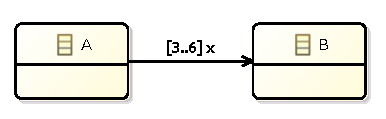
\includegraphics{images/04_transformation_framework/type_models_combination/fieldsig_combine_tmod1.pdf}
        \caption{First type model $Tm_A$}
        \label{fig:transformation_framework:type_models_and_type_graphs:combining_type_models:fieldsig_combine_tmod1}
    \end{subfigure}
    \begin{subfigure}{0.45\textwidth}
        \centering
        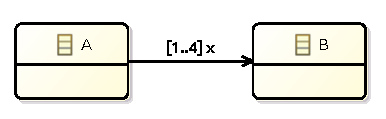
\includegraphics{images/04_transformation_framework/type_models_combination/fieldsig_combine_tmod2.pdf}
        \caption{Second type model $Tm_A$}
        \label{fig:transformation_framework:type_models_and_type_graphs:combining_type_models:fieldsig_combine_tmod2}
    \end{subfigure}
    \par\medskip
    \begin{subfigure}{\textwidth}
        \centering
        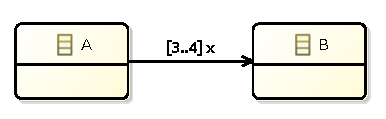
\includegraphics{images/04_transformation_framework/type_models_combination/fieldsig_combine_tmod12.pdf}
        \caption{Combined type model $Tm_{AB}$}
        \label{fig:transformation_framework:type_models_and_type_graphs:combining_type_models:fieldsig_combine_tmod12}
    \end{subfigure}
    \caption{Combination of field signatures when field is present in both type models}
    \label{fig:transformation_framework:type_models_and_type_graphs:combining_type_models:fieldsig_combine}
\end{figure}

An example of the combination of two field signatures in the case of a field being present in both $Tm_A$ and $Tm_B$ is given in \cref{fig:transformation_framework:type_models_and_type_graphs:combining_type_models:fieldsig_combine}. It is possible to combine the field $\type{x}$, since in both $Tm_A$ and $Tm_B$ field $\type{x}$ references class type $\type{B}$. The multiplicity for both field signatures is different and is combined as defined. The maximum of the lower bounds is taken, which results in $\max(3, 1) = 3$. Furthermore, the minimum of the upper bounds is taken, which results in $\min(6, 4) = 4$. Therefore the multiplicity of $\type{x}$ in $Tm_{AB}$ will become $3..4$.

Besides a function for field signatures, a type model also defines a function for constant types. The combination of constant types is discussed in the next definition.

\begin{defin}[Combination function for constant types]
\label{defin:transformation_framework:type_models_and_type_graphs:combining_type_models:consttype_combine}
$\mathrm{consttype\_\!combine}$ is a partial function on two type models which returns a new function \\$Constant_{Tm_{AB}} \Rightarrow Type_{Tm_{AB}}$. It is defined as follows:
\begin{multline*}
    \mathrm{consttype\_\!combine}(Tm_{A}, Tm_{B}, c) = \\
        \begin{cases}
        \mathrm{ConstType}_{Tm_A}(c) & \mathrm{if}\ c \in Constant_{Tm_A} \cap Constant_{Tm_B} \land \mathrm{ConstType}_{Tm_A}(c) = \mathrm{ConstType}_{Tm_B}(c) \\
        \mathrm{ConstType}_{Tm_A}(c) & \mathrm{if}\ c \in Constant_{Tm_A} \setminus Constant_{Tm_B} \\
        \mathrm{ConstType}_{Tm_B}(c) & \mathrm{if}\ c \in Constant_{Tm_B} \setminus Constant_{Tm_A}
    \end{cases}
\end{multline*}
\isabellelref{tmod_combine_const_type}{Ecore.Type_Model_Combination}
\end{defin}

The definition of the combination of constant types is similar to the combination of field signatures. The combination of constant types is less complicated because there is no notion of multiplicities involved. By definition, if a constant only occurs in $Tm_{A}$, the constant type of $Tm_{A}$ is copied. For constants that only occur in $Tm_{B}$, the constant type of $Tm_{B}$ is copied. In case that a constant occurs in both $Tm_{A}$ and $Tm_{B}$, the constant is copied if the constant types for that constant are the same in both $Tm_{A}$ and $Tm_{B}$.

The last definition that remains to be given is the definition of combining the set of properties. The set of properties cannot be united by merely taking the union of $Prop_{Tm_A}$ and $Prop_{Tm_B}$ since this might invalidate the satisfaction of these properties on the level of an instance graph. Instead, the inductive set $\mathrm{prop\_\!combine}$ is defined to specify under which circumstances a property can be combined.

\begin{defin}[Combination of model properties]
\label{defin:transformation_framework:type_models_and_type_graphs:combining_type_models:prop_combine}
$\mathrm{prop\_\!combine}(Tm_A, Tm_B)$ is defined as a subset of $Prop_{Tm_A} \cup Prop_{Tm_B}$. The contents of the set are then defined as follows:

For $\type{abstract}$ properties:
\begin{mathpar}
    \inferrule{[ \type{abstract}, c ] \in Prop_{Tm_A} \\ c \not\in Class_{Tm_B}}{[ \type{abstract}, c ] \in \mathrm{prop\_\!combine}(Tm_A, Tm_B)}
    \and
    \inferrule{[ \type{abstract}, c ] \in Prop_{Tm_B} \\ c \not\in Class_{Tm_A}}{[ \type{abstract}, c ] \in \mathrm{prop\_\!combine}(Tm_A, Tm_B)}
    \and
    \inferrule{[ \type{abstract}, c ] \in Prop_{Tm_A} \\ [ \type{abstract}, c ] \in Prop_{Tm_B}}{[ \type{abstract}, c ] \in \mathrm{prop\_\!combine}(Tm_A, Tm_B)}
\end{mathpar}

For $\type{containment}$ properties:
\begin{mathpar}
    \inferrule{[ \type{containment}, r ]\in Prop_{Tm_A}}{[ \type{containment}, r ]\in \mathrm{prop\_\!combine}(Tm_A, Tm_B)}
    \and
    \inferrule{[ \type{containment}, r ]\in Prop_{Tm_B}}{[ \type{containment}, r ]\in \mathrm{prop\_\!combine}(Tm_A, Tm_B)}
\end{mathpar}

For $\type{defaultValue}$ properties:
\begin{mathpar}
    \inferrule{[ \type{defaultValue}, f, v ]\in Prop_{Tm_A} \\ f \not\in Field_{Tm_B}}{[ \type{defaultValue}, f, v ]\in \mathrm{prop\_\!combine}(Tm_A, Tm_B)}
    \and
    \inferrule{[ \type{defaultValue}, f, v ]\in Prop_{Tm_B} \\ f \not\in Field_{Tm_A}}{[ \type{defaultValue}, f, v ]\in \mathrm{prop\_\!combine}(Tm_A, Tm_B)}
    \and
    \inferrule{[ \type{defaultValue}, f, v ]\in Prop_{Tm_A} \\ [ \type{defaultValue}, f, v ]\in Prop_{Tm_B}}{[ \type{defaultValue}, f, v ]\in \mathrm{prop\_\!combine}(Tm_A, Tm_B)}
\end{mathpar}

For $\type{identity}$ properties:
\begin{mathpar}
    \inferrule{[ \type{identity}, c, A ]\in Prop_{Tm_A} \\ c \not\in Class_{Tm_B}}{[ \type{identity}, c, A ]\in \mathrm{prop\_\!combine}(Tm_A, Tm_B)}
    \and
    \inferrule{[ \type{identity}, c, A ]\in Prop_{Tm_B} \\ c \not\in Class_{Tm_A}}{[ \type{identity}, c, A ]\in \mathrm{prop\_\!combine}(Tm_A, Tm_B)}
    \and
    \inferrule{[ \type{identity}, c, A ]\in Prop_{Tm_A} \\ [ \type{identity}, c, A ]\in Prop_{Tm_B}}{[ \type{identity}, c, A ]\in \mathrm{prop\_\!combine}(Tm_A, Tm_B)}
\end{mathpar}

For $\type{keyset}$ properties:
\begin{mathpar}
    \inferrule{[ \type{keyset}, r, A ]\in Prop_{Tm_A} \\ r \not\in Field_{Tm_B}}{[ \type{keyset}, r, A ]\in \mathrm{prop\_\!combine}(Tm_A, Tm_B)}
    \and
    \inferrule{[ \type{keyset}, r, A ]\in Prop_{Tm_B} \\ r \not\in Field_{Tm_A}}{[ \type{keyset}, r, A ]\in \mathrm{prop\_\!combine}(Tm_A, Tm_B)}
    \and
    \inferrule{[ \type{keyset}, r, A ]\in Prop_{Tm_A} \\ [ \type{keyset}, r, A ]\in Prop_{Tm_B}}{[ \type{keyset}, r, A ]\in \mathrm{prop\_\!combine}(Tm_A, Tm_B)}
\end{mathpar}

For $\type{opposite}$ properties:
\begin{mathpar}
    \inferrule{[ \type{opposite}, r1, r2 ]\in Prop_{Tm_A} \\ r1 \not\in Field_{Tm_B} \\ r2 \not\in Field_{Tm_B}}{[ \type{opposite}, r1, r2 ]\in \mathrm{prop\_\!combine}(Tm_A, Tm_B)}
    \and
    \inferrule{[ \type{opposite}, r1, r2 ]\in Prop_{Tm_B} \\ r1 \not\in Field_{Tm_A} \\ r2 \not\in Field_{Tm_A}}{[ \type{opposite}, r1, r2 ]\in \mathrm{prop\_\!combine}(Tm_A, Tm_B)}
    \and
    \inferrule{[ \type{opposite}, r1, r2 ]\in Prop_{Tm_A} \\ [ \type{opposite}, r1, r2 ]\in Prop_{Tm_B}}{[ \type{opposite}, r1, r2 ]\in \mathrm{prop\_\!combine}(Tm_A, Tm_B)}
\end{mathpar}

For $\type{readonly}$ properties:
\begin{mathpar}
    \inferrule{[ \type{readonly}, f ] \in Prop_{Tm_A} \\ f \not\in Field_{Tm_B}}{[ \type{readonly}, f ] \in \mathrm{prop\_\!combine}(Tm_A, Tm_B)}
    \and
    \inferrule{[ \type{readonly}, f ] \in Prop_{Tm_B} \\ f \not\in Field_{Tm_A}}{[ \type{readonly}, f ] \in \mathrm{prop\_\!combine}(Tm_A, Tm_B)}
    \and
    \inferrule{[ \type{readonly}, f ] \in Prop_{Tm_A} \\ [ \type{readonly}, f ] \in Prop_{Tm_B}}{[ \type{readonly}, f ] \in \mathrm{prop\_\!combine}(Tm_A, Tm_B)}
\end{mathpar}
\isabellelref{tmod_combine_prop}{Ecore.Type_Model_Combination}
\end{defin}

As can be seen from the definition of $\mathrm{prop\_\!combine}(Tm_A, Tm_B)$, properties are only copied under specific circumstances. For $\type{abstract}$ properties, it holds that a class is only abstract in the combination of $Tm_A$ and $Tm_B$ if the class is abstract in both $Tm_A$ and $Tm_B$ or if the class is abstract in one of them, and the class does not occur in the other. Intuitively, this makes sense for correctness. If a class is abstract in both type models, there will not be instances of that class in any of the combined instance models type by those type models. The same holds if the class only occurs in one of the type models, as an instance model cannot contain an instance of a class that is not present in its type model.

For the containment property, it holds that the containment property is always copied over. There are no other conditions here. If there is a containment property in $Prop_{Tm_A} \cup Prop_{Tm_B}$ it will also be in the combination of $Tm_A$ and $Tm_B$.

A default value property is copied over from one of the type models if the other type model does not have the corresponding field defined. Furthermore, a default value may be in the combination of properties of $Tm_A$ and $Tm_B$ if the field occurs in both, and both have the same constant set as the default value for the field. Intuitively, this last requirement makes sense. If we set a default value for a field within a type model, it should not change after combining the type model with another type model, as instance models might depend on the default value set for that field.

Identity properties follow a similar pattern to default value properties. An identity is copied over from one of the type models if the corresponding class is not defined in the other type model. Furthermore, an identity can be preserved if it is set for the same class and attributes in both type models. Again, intuitively, this is the desired solution. If a type model has a class of which a set of attributes can uniquely define the instances, then this should also be the case after the combination with another type model. Merging two sets of attributes might have preserved the identity property as well, but this would be a questionable decision from a practical standpoint, as this means that the identity of instances changes, which makes no sense in real-world scenarios.

The argumentation for identity properties also holds for keyset properties. Therefore these follow a similar pattern, in which the keyset properties of a type model are only copied if the corresponding field does not occur in the other type model, or if the keyset property for a field occurs with the same attributes in both type models.

The opposite property is preserved if it occurs in a type model, but the other type model does not define both of the corresponding fields. Alternatively, the property is preserved if it occurs in both type models with the same fields. All different ways to combine an opposite property would result in an invalid type model according to \cref{defin:formalisations:ecore_formalisation:type_models:type_model_consistency}, which is undesired.

The read-only properties follow a similar pattern to the abstract properties. If a field is read-only in both type models, then it is read-only in the combination. Furthermore, if a field is read-only in one of the type models and the field is not defined in the other type model, then the read-only property can be copied too.

\begin{figure}
    \centering
    \begin{subfigure}{\textwidth}
        \centering
        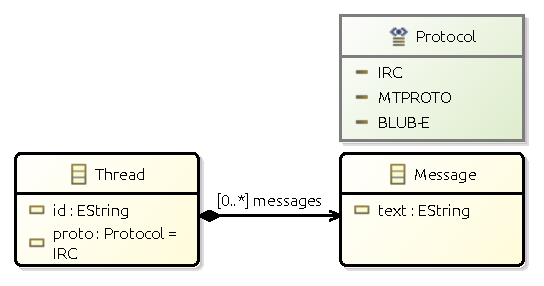
\includegraphics{images/04_transformation_framework/type_models_combination/chat_partial2.pdf}
        \caption{The chat application model $Tm_{Chat}$}
        \label{fig:transformation_framework:type_models_and_type_graphs:combining_type_models:combine_example_tmod1}
    \end{subfigure}
    \par\medskip
    \begin{subfigure}{\textwidth}
        \centering
        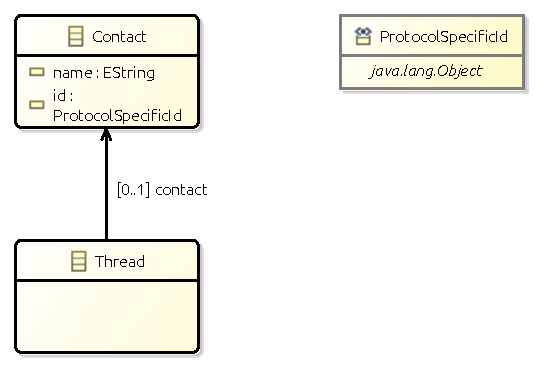
\includegraphics{images/04_transformation_framework/type_models_combination/chat_partial1.pdf}
        \caption{The contact extension model $Tm_{Extension}$}
        \label{fig:transformation_framework:type_models_and_type_graphs:combining_type_models:combine_example_tmod2}
    \end{subfigure}
    \par\medskip
    \begin{subfigure}{\textwidth}
        \centering
        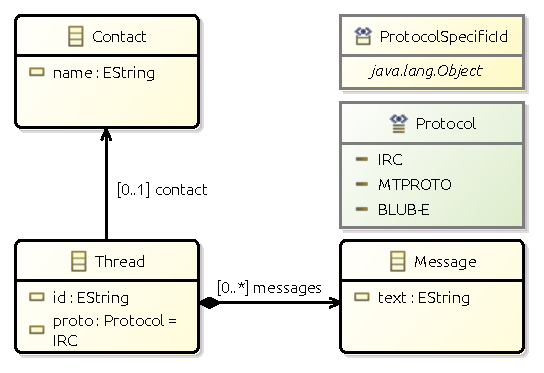
\includegraphics{images/04_transformation_framework/type_models_combination/chat_combined.pdf}
        \caption{The extended chat application model $Tm_{ChatExt}$}
        \label{fig:transformation_framework:type_models_and_type_graphs:combining_type_models:combine_example_tmod12}
    \end{subfigure}
    \caption{Example of the combination of type models}
    \label{fig:transformation_framework:type_models_and_type_graphs:combining_type_models:combine_example}
\end{figure}

With all definitions in place, it is possible to provide a larger example. Suppose the model of a multi-protocol chat application. It consists of $\type{Thread}$s of $\type{Message}$s. Since the application is multi-protocol, each $\type{Thread}$ can use one of the supported $\type{Protocol}$s. The formal definition of the model of such an application could be as follows:

\begin{align*}
Tm_{Chat} =\ &\langle&
Class =\ &\{ \type{.Message}, \type{.Thread} \} \\&&
Enum =\ &\{ \type{.Protocol} \} \\&&
UserDataType =\ &\{\} \\&&
Field =\ &\{
( \type{.Message}, \type{text} ), 
( \type{.Thread}, \type{id} ), 
( \type{.Thread}, \type{messages} ), 
( \type{.Thread}, \type{proto} )\} \\&&
\mathrm{FieldSig} =\ &\big\{
\big( ( \type{.Message}, \type{text} ), ( \type{string}, 1..1 ) \big), \big( ( \type{.Thread}, \type{id} ), ( \type{string}, 1..1 ) \big),\\&&& 
\big( ( \type{.Thread}, \type{messages} ), ( [ \type{seqof}, !\type{.Message} ], 0..\mstar ) \big),\\&&& 
\big( ( \type{.Thread}, \type{proto} ), ( \type{.Protocol}, 1..1 ) \big) \big)
\big\} \\&&
EnumValue =\ &\{
( \type{.Protocol}, \type{IRC} ), 
( \type{.Protocol}, \type{MTPROTO} ), 
( \type{.Protocol}, \type{BLUB\!-\!E} )\} \\&&
Inh =\ &\{\} \\&&
Prop =\ &\big\{
\big( \type{identity}, \type{.Message}, \{( \type{.Thread}, \type{id} )\} \big)
\big\} \\&&
Constant =\ &\{\} \\&&
\mathrm{ConstType} =\ &\{\}
\\&\rangle
\end{align*}

An visual representation of $Tm_{Chat}$ is included as  \cref{fig:transformation_framework:type_models_and_type_graphs:combining_type_models:combine_example_tmod1}. Now, assume a model that represents an extension to this application, adding support for $\type{Contact}$s. Each thread can belong to a $\type{Contact}$. A $\type{Contact}$ has a name and some identifier that is protocol specific. For that identifier, the user-defined data type $\type{ProtocolSpecificId}$ is introduced. This extension could formally be defined as:

\begin{align*}
Tm_{Extension} =\ &\langle&
Class =\ &\{ \type{.Contact}, \type{.Thread} \} \\&&
Enum =\ &\{\} \\&&
UserDataType =\ &\{ \type{.ProtocolSpecificId} \} \\&&
Field =\ &\{
( \type{.Contact}, \type{name} ), 
( \type{.Contact}, \type{id} ), 
( \type{.Thread}, \type{contact} )\} \\&&
\mathrm{FieldSig} =\ &\big\{
\big( ( \type{.Contact}, \type{name} ), ( \type{string}, 1..1 ) \big),\\&&& \big( ( \type{.Contact}, \type{id} ), ( \type{.ProtocolSpecificId}, 1..1 ) \big),\\&&& 
\big( ( \type{.Thread}, \type{contact} ), ( ?\type{.Contact}, 0..1 ) \big) \big)
\big\} \\&&
EnumValue =\ &\{\} \\&&
Inh =\ &\{\} \\&&
Prop =\ &\big\{
\big( \type{identity}, \type{.Contact}, \{( \type{.Contact}, \type{id} )\} \big)
\big\} \\&&
Constant =\ &\{\} \\&&
\mathrm{ConstType} =\ &\{\}
\\&\rangle
\end{align*}

The visual representation of the extension is included as \cref{fig:transformation_framework:type_models_and_type_graphs:combining_type_models:combine_example_tmod2}. Now, using \cref{defin:transformation_framework:type_models_and_type_graphs:combining_type_models:combine}, it is possible to combine these models into one model. This will yield the following model:

\begin{align*}
Tm_{ChatExt} =\ &\langle&
Class =\ &\{ \type{.Contact}, \type{.Message}, \type{.Thread} \} \\&&
Enum =\ &\{ \type{.Protocol} \} \\&&
UserDataType =\ &\{ \type{.ProtocolSpecificId} \} \\&&
Field =\ &\{
( \type{.Contact}, \type{name} ), 
( \type{.Contact}, \type{id} ),
( \type{.Message}, \type{text} ),\\&&&
( \type{.Thread}, \type{contact} ),
( \type{.Thread}, \type{id} ),
( \type{.Thread}, \type{messages} ),\\&&& 
( \type{.Thread}, \type{proto} )\} \\&&
\mathrm{FieldSig} =\ &\big\{
\big( ( \type{.Contact}, \type{name} ), ( \type{string}, 1..1 ) \big),\\&&& \big( ( \type{.Contact}, \type{id} ), ( \type{.ProtocolSpecificId}, 1..1 ) \big),\\&&& 
\big( ( \type{.Message}, \type{text} ), ( \type{string}, 1..1 ) \big),\\&&&
\big( ( \type{.Thread}, \type{contact} ), ( ?\type{.Contact}, 0..1 ) \big) \big),\\&&&
\big( ( \type{.Thread}, \type{id} ), ( \type{string}, 1..1 ) \big),\\&&& 
\big( ( \type{.Thread}, \type{messages} ), ( [ \type{seqof}, !\type{.Message} ], 0..\mstar ) \big),\\&&& 
\big( ( \type{.Thread}, \type{proto} ), ( \type{.Protocol}, 1..1 ) \big) \big)
\big\} \\&&
EnumValue =\ &\{
( \type{.Protocol}, \type{IRC} ), 
( \type{.Protocol}, \type{MTPROTO} ), 
( \type{.Protocol}, \type{BLUB\!-\!E} )\} \\&&
Inh =\ &\{\} \\&&
Prop =\ &\big\{
\big( \type{identity}, \type{.Contact}, \{( \type{.Contact}, \type{id} )\} \big),\\&&&
\big( \type{identity}, \type{.Message}, \{( \type{.Thread}, \type{id} )\} \big)
\big\} \\&&
Constant =\ &\{\} \\&&
\mathrm{ConstType} =\ &\{\}
\\&\rangle
\end{align*}

A visual representation of this combined model is included as \cref{fig:transformation_framework:type_models_and_type_graphs:combining_type_models:combine_example_tmod12}. The example perfectly shows why the combination of type models is useful: It allows for building larger models out of smaller building blocks. This is the exact goal of this definition within the transformation framework.

Although the definitions of the combination of type models are given, no mathematical properties or theorems are defined yet. Some mathematical properties hold for the combination of type models, that will be presented in the following theorems.

\begin{thm}[Commutativity of the combination of type models]
\label{defin:transformation_framework:type_models_and_type_graphs:combining_type_models:tmod_combine_commute}
Assume that $Tm_A$ and $Tm_B$ are type models, then the $\mathrm{combine}$ function is commutative:
\begin{equation*}
    \mathrm{combine}(Tm_A, Tm_B) = \mathrm{combine}(Tm_B, Tm_A)
\end{equation*}
\isabellelref{tmod_combine_commute}{Ecore.Type_Model_Combination}
\end{thm}

\begin{thm}[Associativity of the combination of type models]
\label{defin:transformation_framework:type_models_and_type_graphs:combining_type_models:tmod_combine_assoc}
Assume that $Tm_A$, $Tm_B$ and $Tm_C$ are type models, then the $\mathrm{combine}$ function is associative:
\begin{equation*}
    \mathrm{combine}(\mathrm{combine}(Tm_A, Tm_B), Tm_C) = \mathrm{combine}(Tm_A, \mathrm{combine}(Tm_B, Tm_C))
\end{equation*}
\isabellelref{tmod_combine_assoc}{Ecore.Type_Model_Combination}
\end{thm}

\begin{thm}[Idempotence of the combination of type models]
\label{defin:transformation_framework:type_models_and_type_graphs:combining_type_models:tmod_combine_idemp}
Assume that $Tm_A$ is a type model and that it is consistent in the sense of \cref{defin:formalisations:ecore_formalisation:type_models:type_model_consistency}. Then the following property holds:
\begin{equation*}
    \mathrm{combine}(Tm_A, Tm_A) = Tm_A
\end{equation*}
\isabellelref{tmod_combine_idemp_alt}{Ecore.Type_Model_Combination}
\end{thm}

These properties follow directly from \cref{defin:transformation_framework:type_models_and_type_graphs:combining_type_models:combine}, but the corresponding proofs will not be included here. It should be noted that these properties are indeed proven correct as part of this thesis, and the corresponding proofs are validated within Isabelle.

Besides these properties, the combination of type models also has an identity element. The empty type model represents this identity element, but it needs to be defined first:

\begin{defin}[Empty type model]
\label{defin:transformation_framework:type_models_and_type_graphs:combining_type_models:empty_type_model}
Let $Tm_{\epsilon}$ be the empty type model. $Tm_{\epsilon}$ is defined as:
\begin{align*}
Tm_{\epsilon} = \langle&
Class = \{\} \\&
Enum = \{\} \\&
UserDataType = \{\} \\&
Field = \{\} \\&
\mathrm{FieldSig} = undefined \\&
EnumValue = \{\} \\&
Inh = \{\} \\&
Prop = \{\} \\&
Constant = \{\} \\&
\mathrm{ConstType} = undefined\rangle
\end{align*}
\end{defin}

\begin{thm}[Correctness of the empty type model]
\label{defin:transformation_framework:type_models_and_type_graphs:combining_type_models:tmod_empty_correct}
The empty type model, $Tm_{\epsilon}$, is consistent with respect to
\cref{defin:formalisations:ecore_formalisation:type_models:type_model_consistency}.
\isabellelref{tmod_empty_correct}{Ecore.Type_Model}
\end{thm}

The proof for the correctness of the empty type model is trivial. Still, a validated version of this proof can be found within the Isabelle theories of this thesis.

As mentioned earlier, the empty type model acts as an identity element when combining two type models. The following theorem specifies this behaviour.

\begin{thm}[Identity of the combination of type models]
\label{defin:transformation_framework:type_models_and_type_graphs:combining_type_models:tmod_combine_identity}
Assume that $Tm_A$ is a type model and that it is consistent in the sense of \cref{defin:formalisations:ecore_formalisation:type_models:type_model_consistency}. Then $Tm_{\epsilon}$ acts as an identity element in the combination function:
\begin{equation*}
    \mathrm{combine}(Tm_{\epsilon}, Tm_A) = Tm_A
\end{equation*}
\isabellelref{tmod_combine_identity_alt}{Ecore.Type_Model_Combination}
\end{thm}

Once more, the proof of this theorem follows directly from the definition. Therefore, the corresponding proof will not be included here, but a validated version can be found within the Isabelle theories of this thesis.

A final desired property for the combination of type models is a correctness property. \cref{defin:transformation_framework:type_models_and_type_graphs:combining_type_models:tmod_combine_correct} defines the theorem under which the combination of type models is a consistent type model. Please note that this theorem is a generic theorem, which does not take into account that the type models are mostly distinct.

\begin{thm}[Consistency of the combination of type models]
\label{defin:transformation_framework:type_models_and_type_graphs:combining_type_models:tmod_combine_correct}
Assume that $Tm_A$ and $Tm_B$ are consistent type models in the sense of \cref{defin:formalisations:ecore_formalisation:type_models:type_model_consistency}. Furthermore, assume the following properties:
\begin{itemize}
    \item For all shared fields, the type is the same in both type models: $\forall f \in Field_{Tm_A} \cap Field_{Tm_B}\!: \mathrm{type}_{Tm_A}(f) = \mathrm{type}_{Tm_B}(f)$
    \item For all shared fields, the combination of the multiplicities is a valid multiplicity: $\forall f \in Field_{Tm_A} \cap Field_{Tm_B}\!: \max\big(\mathrm{lower}(\mathrm{FieldSig}_{Tm_A}(f)), \mathrm{lower}(\mathrm{FieldSig}_{Tm_B}(f))\big) .. \min\big(\mathrm{upper}(\mathrm{FieldSig}_{Tm_A}(f)),$\\ $\mathrm{upper}(\mathrm{FieldSig}_{Tm_B}(f))\big) \in \mathbb{M}$
    \item For all shared constants, the constant type is the same in both models: $\forall f \in Constant_{Tm_A} \cap Constant_{Tm_B}\!: \mathrm{ConstType}_{Tm_A}(f) = \mathrm{ConstType}_{Tm_B}(f)$
    \item Identifiers used for a class in $Tm_A$ cannot be used for an enumeration type or user-defined data type in $Tm_B$: $\forall c \in Class_{Tm_A}\!: c \not\in Enum_{Tm_B} \land c \not\in UserDataType_{Tm_B}$.
    \item Identifiers used for a class in $Tm_B$ cannot be used for an enumeration type or user-defined data type in $Tm_A$: $\forall c \in Class_{Tm_B}\!: c \not\in Enum_{Tm_A} \land c \not\in UserDataType_{Tm_A}$.
    \item Identifiers used for an enumeration type in $Tm_A$ cannot be used for a class or user-defined data type in $Tm_B$: $\forall c \in Enum_{Tm_A}\!: c \not\in Class_{Tm_B} \land c \not\in UserDataType_{Tm_B}$.
    \item Identifiers used for an enumeration type in $Tm_B$ cannot be used for a class or user-defined data type in $Tm_A$: $\forall c \in Enum_{Tm_B}\!: c \not\in Class_{Tm_A} \land c \not\in UserDataType_{Tm_A}$.
    \item Identifiers from $Tm_A$ may not be in the namespace of an identifier in $Tm_B$: $\forall x \in Class_{Tm_A} \cup Enum_{Tm_A} \cup UserDataType_{Tm_A}; y \in Class_{Tm_B} \cup Enum_{Tm_B} \cup UserDataType_{Tm_B}\!:$\\$x \text{ not in the namespace of } y$
    \item Identifiers from $Tm_B$ may not be in the namespace of an identifier in $Tm_A$: $\forall x \in Class_{Tm_B} \cup Enum_{Tm_B} \cup UserDataType_{Tm_B}; y \in Class_{Tm_A} \cup Enum_{Tm_A} \cup UserDataType_{Tm_A}\!:$\\$x \text{ not in the namespace of } y$
    \item The transitive closure of the inheritance relation is irreflexive: $(Inh_{Tm_A} \cup Inh_{Tm_B})^+$ is irreflexive
    \item For any superclass with an identity, the identity of the subclasses must be a superset of the identity of the superclass: $\forall c_1\ c_2\ A_1\ A_2\!: [ \type{identity}, c_1, A_1 ] \in \mathrm{prop\_\!combine}(Tm_A, Tm_B) \land [ \type{identity}, c_2, A_2 ] \in \mathrm{prop\_\!combine}(Tm_A, Tm_B) \land c_1 \neq c_2\ \land\ !c_1 \not\sqsubseteq_{Tm_A}\ !c_2\ \land\ !c_1 \not\sqsubseteq_{Tm_B}\ !c_2\ \land\ !c_1 \sqsubseteq_{\mathrm{combine}(Tm_A, Tm_B)}\ !c_2 \implies A \subseteq B$
    \item For all shared fields, if $Tm_{A}$ defines a default value, $Tm_{B}$ should define the same default value, and vice versa: $\forall f \in Field_{Tm_A} \cap Field_{Tm_B}\!: [ \type{defaultValue}, f, v ] \in Prop_{Tm_A} \Longleftrightarrow [ \type{defaultValue}, f, v ] \in Prop_{Tm_B}$.
    \item For all shared classes, if $Tm_{A}$ defines a identity, $Tm_{B}$ should define the same identity, and vice versa: $\forall c \in Class_{Tm_A} \cap Class_{Tm_B}\!: [ \type{identity}, c, A ] \in Prop_{Tm_A} \Longleftrightarrow [ \type{identity}, c, A ] \in Prop_{Tm_B}$.
    \item For all shared fields, if $Tm_{A}$ defines a keyset, $Tm_{B}$ should define the same keyset, and vice versa: $\forall r \in Field_{Tm_A} \cap Field_{Tm_B}\!: [ \type{keyset}, r, A ] \in Prop_{Tm_A} \Longleftrightarrow [ \type{keyset}, r, A ] \in Prop_{Tm_B}$.
    \item For all shared fields, if $Tm_{A}$ defines an opposite property, $Tm_{B}$ should define the same opposite property, and vice versa: $\forall r \in Field_{Tm_A} \cap Field_{Tm_B}\!: [ \type{opposite}, r, r' ] \in Prop_{Tm_A} \Longleftrightarrow [ \type{opposite}, r, r' ] \in Prop_{Tm_B}$
\end{itemize}

Then $\mathrm{combine}(Tm_A, Tm_B)$ is a consistent type model in the sense of \cref{defin:formalisations:ecore_formalisation:type_models:type_model_consistency}
\isabellelref{tmod_combine_correct}{Ecore.Type_Model_Combination}
\end{thm}

\begin{proof}
To proof that $\mathrm{combine}(Tm_A, Tm_B)$ is a consistent type model, it needs to be shown that\\ $\mathrm{combine}(Tm_A, Tm_B)$ gives rise to a valid structure for a type model and that \cref{defin:formalisations:ecore_formalisation:type_models:type_model_consistency} holds. For readability, define $Tm_{AB}$ to be $\mathrm{combine}(Tm_A, Tm_B)$.

\emph{Structural properties}
\begin{itemize}
    \item All elements of $Class_{Tm_{AB}}$ are elements of $Id$.
    
    Follows from $Class_{Tm_A} \subseteq Id$ and $Class_{Tm_B} \subseteq Id$.
    
    
    \item All elements of $Enum_{Tm_{AB}}$ are elements of $Id$.
    
    Follows from $Enum_{Tm_A} \subseteq Id$ and $Enum_{Tm_B} \subseteq Id$.
    
    
    \item All elements of $UserDataType_{Tm_{AB}}$ are elements of $Id$.
    
    Follows from $UserDataType_{Tm_A} \subseteq Id$ and $UserDataType_{Tm_B} \subseteq Id$.
    
    
    \item All elements of $Field_{Tm_{AB}}$ are elements of $(Class_{Tm_{AB}} \times Name)$.
    
    Follows from $Field_{Tm_A} \subseteq (Class_{Tm_A} \times Name)$ and $Field_{Tm_B} \subseteq (Class_{Tm_B} \times Name)$. To complete the proof, use $Class_{Tm_{AB}} = Class_{Tm_A} \cup Class_{Tm_B}$.
    
    
    \item For each field $f$, $\mathrm{FieldSig}_{Tm_{AB}}(f)$ must be an element of $(Type_{Tm_{AB}} \times \mathbb{M})$.
    
    First, note that $Type_{Tm_{AB}} = Type_{Tm_A} \cup Type_{Tm_B}$\\(see \isabelleref{tmod_combine_type}{Ecore.Type_Model_Combination}).
    
    If $f \in Field_{Tm_A} \setminus Field_{Tm_B}$, then $\mathrm{FieldSig}_{Tm_{AB}}(f) \in (Type_{Tm_{AB}} \times \mathbb{M})$.
    
    Similarly, if $f \in Field_{Tm_B} \setminus Field_{Tm_A}$, then $\mathrm{FieldSig}_{Tm_{AB}}(f) \in (Type_{Tm_{AB}} \times \mathbb{M})$. 
    
    If $f \in Field_{Tm_A} \cap Field_{Tm_B}$, then $\mathrm{type}_{Tm_A}(f) = \mathrm{type}_{Tm_B}(f)$ by assumption. Also, the combined multiplicity is correct by assumption. Therefore $\mathrm{FieldSig}_{Tm_{AB}}(f) \in (Type_{Tm_{AB}} \times \mathbb{M})$.
    
    
    \item All elements of $EnumValue_{Tm_{AB}}$ are elements of $(Enum_{Tm_{AB}} \times Name)$.
    
    Follows from $EnumValue_{Tm_A} \subseteq (Enum_{Tm_A} \times Name)$ and $EnumValue_{Tm_B} \subseteq (Enum_{Tm_B} \times Name)$. To complete the proof, use $Enum_{Tm_{AB}} = Enum_{Tm_A} \cup Enum_{Tm_B}$.
    
    
    \item All elements of $Inh_{Tm_{AB}}$ are elements of $(Class_{Tm_{AB}} \times Class_{Tm_{AB}})$.
    
    Follows from $Inh_{Tm_A} \subseteq (Class_{Tm_A} \times Class_{Tm_A})$ and $Inh_{Tm_B} \subseteq (Class_{Tm_B} \times Class_{Tm_B})$. Furthermore, $Class_{Tm_{AB}} = Class_{Tm_A} \cup Class_{Tm_B}$.
    
    
    \item All elements of $Prop_{Tm_{AB}}$ are elements of $Property_{Tm_{AB}}$.
    
    Make a case distinction for the different possible properties.
    \begin{itemize}
        \item For $[ \type{abstract}, c ] \in Prop_{Tm_{AB}}$, use the fact that $c \in Class_{Tm_A} \cup Class_{Tm_B}$. Therefore, $[ \type{abstract}, c ] \in Property_{Tm_{AB}}$.
        
        \item For $[ \type{containment}, r ] \in Prop_{Tm_{AB}}$, use the fact that $Rel_{Tm_{AB}} = Rel_{Tm_A} \cup Rel_{Tm_B}$ (see \isabelleref{tmod_combine_rel}{Ecore.Type_Model_Combination}). Then have $[ \type{containment}, r ] \in Property_{Tm_{AB}}$.
        
        \item For $[ \type{defaultValue}, f, v ] \in Prop_{Tm_{AB}}$, use the fact that $f \in Field_{Tm_A} \cup Field_{Tm_B}$ and $v \in Constant_{Tm_A} \cup Constant_{Tm_B}$. Using a case disinction on the combination of properties, it is possible to show that $\mathrm{ConstType}_{Tm_{AB}}(v) \sqsubseteq_{Tm_{AB}} \mathrm{type}_{Tm_{AB}}(f)$. Therefore, $[ \type{defaultValue}, f, v ] \in Property_{Tm_{AB}}$.
        
        \item For $[ \type{identity}, c, A ] \in Prop_{Tm_{AB}}$, use the fact that $c \in Class_{Tm_A} \cup Class_{Tm_B}$ and $A \subseteq fields_{Tm_A} \lor A \subseteq fields_{Tm_B}$. Then have that $A \subseteq fields_{Tm_{AB}}$ Therefore, $[ \type{identity}, c, A ] \in Property_{Tm_{AB}}$.
        
        \item For $[ \type{keyset}, r, A ] \in Prop_{Tm_{AB}}$, use the fact that $Rel_{Tm_{AB}} = Rel_{Tm_A} \cup Rel_{Tm_B}$ (see \isabelleref{tmod_combine_rel}{Ecore.Type_Model_Combination}) to show $r \in Rel_{Tm_{AB}}$. Also use the fact that $Attr_{Tm_{AB}} = Attr_{Tm_A} \cup Attr_{Tm_B}$ to show $A \subseteq Attr_{Tm_{AB}}$ (see \isabelleref{tmod_combine_attr}{Ecore.Type_Model_Combination}). Because types are preserved after combining, it is possible to show that $\forall f \in A\!: \mathrm{uncontainer}(\mathrm{type}_{Tm_{AB}}(r)) \sqsubseteq_{Tm_{AB}} \mathrm{class}_{Tm_{AB}}(f)$. Furthermore, $\mathrm{type}_{Tm_{AB}}(r) \in (\{ \type{setof}, \type{ordof} \} \times ClassType_{Tm_{AB}})$. Therefore, $[ \type{keyset}, r, A ] \in Property_{Tm_{AB}}$.
        
        \item For $[ \type{opposite}, r, r' ] \in Prop_{Tm_{AB}}$, use the fact that $Rel_{Tm_{AB}} = Rel_{Tm_A} \cup Rel_{Tm_B}$ (see \isabelleref{tmod_combine_rel}{Ecore.Type_Model_Combination}) to show $r \in Rel_{Tm_{AB}}$ and $r' \in Rel_{Tm_{AB}}$. Because types are preserved after combining, it is possible to show that $!c1 \sqsubseteq_{Tm_{AB}} \mathrm{uncontainer}(\mathrm{type}_{Tm_{AB}}(r'))$, $!c2 \sqsubseteq_{Tm_{AB}} \mathrm{uncontainer}(\mathrm{type}_{Tm_{AB}}(r))$,\\ $\mathrm{type}_{Tm_{AB}}(r) \not\in \{ \type{bagof}, \type{seqof} \} \times Type_{Tm_{AB}}$ and finally $type_{Tm_{AB}}(r') \not\in \{ \type{bagof}, \type{seqof} \} \times Type_{Tm_{AB}}$. Therefore, $[ \type{opposite}, r, r' ] \in Property_{Tm_{AB}}$.
        
        \item For $[ \type{readonly}, f ] \in Prop_{Tm_{AB}}$, use the fact that $f \in Field_{Tm_A} \cup Field_{Tm_B}$. Therefore, $[ \type{readonly}, f ] \in Property_{Tm_{AB}}$.
    \end{itemize}
    
    
    \item All elements of $Constant_{Tm_{AB}}$ are elements of $Id$.
    
    Follows from $Constant_{Tm_A} \subseteq Id$ and $Constant_{Tm_B} \subseteq Id$.
    
    
    \item For each constant $c$, $\mathrm{ConstType}_{Tm_{AB}}(c)$ must be an element of $Type_{Tm_{AB}}$.
    
    First, note that $Type_{Tm_{AB}} = Type_{Tm_A} \cup Type_{Tm_B}$\\(see \isabelleref{tmod_combine_type}{Ecore.Type_Model_Combination}).
    
    If $c \in Constant_{Tm_A} \setminus Constant_{Tm_B}$, then $\mathrm{ConstType}_{Tm_{AB}}(f) \in Type_{Tm_{AB}}$.
    
    Similarly, if $c \in Constant_{Tm_B} \setminus Constant_{Tm_A}$, then $\mathrm{ConstType}_{Tm_{AB}}(c) \in Type_{Tm_{AB}}$.
    
    If $c \in Constant_{Tm_A} \cap Constant_{Tm_B}$, then $\mathrm{ConstType}_{Tm_A}(c) = \mathrm{ConstType}_{Tm_B}(c)$ by assumption. Therefore $\mathrm{ConstType}_{Tm_{AB}}(c) \in Type_{Tm_{AB}}$.
    
    
    \item $Class_{Tm_{AB}}$, $DataType$, $Enum_{Tm_{AB}}$ and $UserDataType_{Tm_{AB}}$ are pairwise disjoint.
    
    Notice that $Class_{Tm_{A}}$, $DataType$, $Enum_{Tm_{A}}$, $UserDataType_{Tm_{A}}$ are pairwise disjoint. Also, $Class_{Tm_{B}}$, $DataType$, $Enum_{Tm_{B}}$, $UserDataType_{Tm_{B}}$ are pairwise disjoint.
    
    Use that $Class_{Tm_{AB}} = Class_{Tm_{A}} \cup Class_{Tm_{B}}$, $Enum_{Tm_{AB}} = Enum_{Tm_{A}} \cup Enum_{Tm_{B}}$ and\\ $UserDataType_{Tm_{AB}} = UserDataType_{Tm_{A}} \cup UserDataType_{Tm_{B}}$. Use this to split the possible cases.
    
    Only the case where one element is from $Class_{Tm_{A}} \cup Enum_{Tm_{A}} \cup UserDataType_{Tm_{A}}$ and one element is from $Class_{Tm_{B}} \cup Enum_{Tm_{B}} \cup UserDataType_{Tm_{B}}$ cannot be proven directly. For this case, the proof follows from the assumptions.
    
    
    \item None of the elements in $Class_{Tm_{AB}}$, $DataType$, $Enum_{Tm_{AB}}$ and $UserDataType_{Tm_{AB}}$ may be in the namespace of another element in that set.
    
    Use that $Class_{Tm_{AB}} = Class_{Tm_{A}} \cup Class_{Tm_{B}}$, $Enum_{Tm_{AB}} = Enum_{Tm_{A}} \cup Enum_{Tm_{B}}$ and\\ $UserDataType_{Tm_{AB}} = UserDataType_{Tm_{A}} \cup UserDataType_{Tm_{B}}$. Use this to split the possible cases.
    
    It is not possible to directly proof the cases where the identifier comes from $Class_{Tm_{A}} \cup Enum_{Tm_{A}} \cup UserDataType_{Tm_{A}}$ and the namespace comes from $Class_{Tm_{B}} \cup Enum_{Tm_{B}} \cup UserDataType_{Tm_{B}}$. Furthermore, it is also not possible for the cases where the identifier comes from $Class_{Tm_{B}} \cup Enum_{Tm_{B}} \cup UserDataType_{Tm_{B}}$ and the namespace comes from\\ $Class_{Tm_{A}} \cup Enum_{Tm_{A}} \cup UserDataType_{Tm_{A}}$. For these cases, the proof follows from the assumptions.
    
    
    \item $Inh_{Tm_{AB}}$ is an asymmetric relation, of which the transitive closure is irreflexive.
    
    The transitive closure of $Inh_{Tm_{AB}}$ is irreflexive by assumption. Then show that $Inh_{Tm_{AB}}$ is an asymmetric relation using the assumption that the transitive closure of $Inh_{Tm_{AB}}$ is irreflexive.
\end{itemize}

\emph{Consistency properties}
\begin{itemize}
    \item For all $\mathrm{type}_{Tm_{AB}}(f) \in DataType \cup Enum_{Tm_{AB}} \cup UserDataType_{Tm_{AB}} \cup (\type{proper} \times Class_{Tm_{AB}})$, it holds that $\mathrm{lower}_{Tm_{AB}}(f) = 1$.
    
    Use the fact that $\mathrm{type}_{Tm_{AB}}(f) = \mathrm{type}_{Tm_{A}}(f)$ or $\mathrm{type}_{Tm_{AB}}(f) = \mathrm{type}_{Tm_{B}}(f)$.
    
    If $\mathrm{type}_{Tm_{AB}}(f) = \mathrm{type}_{Tm_{A}}(f)$, then $\mathrm{type}_{Tm_{AB}}(f) \in DataType \cup Enum_{Tm_{AB}} \cup UserDataType_{Tm_{AB}} \cup (\type{proper} \times Class_{Tm_{AB}})$ only when $\mathrm{type}_{Tm_{A}}(f) \in DataType \cup Enum_{Tm_{A}} \cup UserDataType_{Tm_{A}} \cup (\type{proper} \times Class_{Tm_{A}})$.
    
    Then if $\mathrm{type}_{Tm_{A}}(f) \in DataType \cup Enum_{Tm_{A}} \cup UserDataType_{Tm_{A}} \cup (\type{proper} \times Class_{Tm_{A}})$, then $\mathrm{lower}_{Tm_{A}}(f) = 1$. As a consequence, it must be that $\mathrm{lower}_{Tm_{AB}}(f) = 1$.
    
    If $\mathrm{type}_{Tm_{AB}}(f) = \mathrm{type}_{Tm_{B}}(f)$, then $\mathrm{type}_{Tm_{AB}}(f) \in DataType \cup Enum_{Tm_{AB}} \cup UserDataType_{Tm_{AB}} \cup (\type{proper} \times Class_{Tm_{AB}})$ only when $\mathrm{type}_{Tm_{B}}(f) \in DataType \cup Enum_{Tm_{B}} \cup UserDataType_{Tm_{B}} \cup (\type{proper} \times Class_{Tm_{B}})$.
    
    Then if $\mathrm{type}_{Tm_{B}}(f) \in DataType \cup Enum_{Tm_{B}} \cup UserDataType_{Tm_{B}} \cup (\type{proper} \times Class_{Tm_{B}})$, then $\mathrm{lower}_{Tm_{B}}(f) = 1$. As a consequence, it must be that $\mathrm{lower}_{Tm_{AB}}(f) = 1$.
    
    
    \item For all $\mathrm{type}_{Tm_{AB}}(f) \in (\type{nullable} \times Class_{Tm_{AB}})$, it holds that $\mathrm{lower}_{Tm_{AB}}(f) = 0$.
    
    Use the fact that $\mathrm{type}_{Tm_{AB}}(f) = \mathrm{type}_{Tm_{A}}(f)$ or $\mathrm{type}_{Tm_{AB}}(f) = \mathrm{type}_{Tm_{B}}(f)$.
    
    If $\mathrm{type}_{Tm_{AB}}(f) = \mathrm{type}_{Tm_{A}}(f)$, then $\mathrm{type}_{Tm_{AB}}(f) \in (\type{nullable} \times Class_{Tm_{AB}})$ only when $\mathrm{type}_{Tm_{A}}(f) \in (\type{nullable} \times Class_{Tm_{A}})$.
    
    Then if $\mathrm{type}_{Tm_{A}}(f) \in (\type{nullable} \times Class_{Tm_{A}})$, then $\mathrm{lower}_{Tm_{A}}(f) = 0$. As a consequence, it must be that $\mathrm{lower}_{Tm_{AB}}(f) = 0$.
    
    If $\mathrm{type}_{Tm_{AB}}(f) = \mathrm{type}_{Tm_{B}}(f)$, then $\mathrm{type}_{Tm_{AB}}(f) \in (\type{nullable} \times Class_{Tm_{AB}})$ only when $\mathrm{type}_{Tm_{B}}(f) \in (\type{nullable} \times Class_{Tm_{B}})$.
    
    Then if $\mathrm{type}_{Tm_{B}}(f) \in (\type{nullable} \times Class_{Tm_{AB}})$, then $\mathrm{lower}_{Tm_{B}}(f) = 0$. As a consequence, it must be that $\mathrm{lower}_{Tm_{AB}}(f) = 0$.
    
    
    \item For all $\mathrm{type}_{Tm_{AB}}(f) \not\in Container_{Tm_{AB}}$, it holds that $\mathrm{upper}_{Tm_{AB}}(f) = 1$.
    
    Use the fact that $\mathrm{type}_{Tm_{AB}}(f) = \mathrm{type}_{Tm_{A}}(f)$ or $\mathrm{type}_{Tm_{AB}}(f) = \mathrm{type}_{Tm_{B}}(f)$.
    
    If $\mathrm{type}_{Tm_{AB}}(f) = \mathrm{type}_{Tm_{A}}(f)$, then $\mathrm{type}_{Tm_{AB}}(f) \not\in Container_{Tm_{AB}}$ only when $\mathrm{type}_{Tm_{A}}(f) \not\in Container_{Tm_{A}}$.
    
    Then if $\mathrm{type}_{Tm_{A}}(f) \not\in Container_{Tm_{A}}$, then $\mathrm{upper}_{Tm_{A}}(f) = 1$. As a consequence, must also be $\mathrm{upper}_{Tm_{AB}}(f) = 1$.
    
    If $\mathrm{type}_{Tm_{AB}}(f) = \mathrm{type}_{Tm_{B}}(f)$, then $\mathrm{type}_{Tm_{AB}}(f) \not\in Container_{Tm_{AB}}$ only when $\mathrm{type}_{Tm_{B}}(f) \not\in Container_{Tm_{B}}$.
    
    Then if $\mathrm{type}_{Tm_{B}}(f) \not\in Container_{Tm_{B}}$, then $\mathrm{upper}_{Tm_{B}}(f) = 1$. As a consequence, must also be $\mathrm{upper}_{Tm_{AB}}(f) = 1$.


    \item $[ \type{containment}, r ] \in Prop_{Tm_{AB}} \land [ \type{opposite}, r, r' ] \in Prop_{Tm_{AB}} \Longrightarrow upper_{Tm_{AB}}(r') = 1$.
    
    Use the fact that $[ \type{containment}, r ] \in Prop_{Tm_{AB}}$ means that $[ \type{containment}, r ] \in Prop_{Tm_{A}}$ or $[ \type{containment}, r ] \in Prop_{Tm_{B}}$
    
    Also use the fact that $[ \type{opposite}, r, r' ] \in Prop_{Tm_{AB}}$ means that $[ \type{opposite}, r, r' ] \in Prop_{Tm_{A}} \setminus Prop_{Tm_{B}}$, $[ \type{opposite}, r, r' ] \in Prop_{Tm_{B}} \setminus Prop_{Tm_{A}}$ or $\type{opposite}, r, r' ] \in Prop_{Tm_{A}} \cap Prop_{Tm_{B}}$.
    
    Based on these two facts, make a case distinction of all 6 possible cases. The case where $[ \type{opposite}, r, r' ] \in Prop_{Tm_{A}} \setminus Prop_{Tm_{B}}$ and $[ \type{containment}, r ] \in Prop_{Tm_{B}}$ is invalid, since $r$ cannot be part of $Field_{Tm_B}$ by definition of the combination of properties. Similarly, the case  $[ \type{opposite}, r, r' ] \in Prop_{Tm_{B}} \setminus Prop_{Tm_{A}}$ and $[ \type{containment}, r ] \in Prop_{Tm_{A}}$ is also invalid.
    
    For the other cases, at least $\mathrm{upper}_{Tm_{A}}(r') = 1$ or $\mathrm{upper}_{Tm_{B}}(r') = 1$. The upper bound of $r$ in the other type model may be larger than $1$. By the definition of the combination of field signatures, $\mathrm{upper}_{Tm_{AB}}(r') = 1$.
    
    
    \item $[ \type{defaultValue}, f, v ] \in Prop_{Tm_{AB}} \land [ \type{defaultValue}, f, v' ] \in Prop_{Tm_{AB}} \Longrightarrow v = v'$.
    
    Use the fact that $[ \type{defaultValue}, f, v ] \in Prop_{Tm_{AB}}$ means that $[ \type{defaultValue}, f, v ] \in Prop_{Tm_{A}} \setminus Prop_{Tm_{B}}$, $[ \type{defaultValue}, f, v ] \in Prop_{Tm_{B}} \setminus Prop_{Tm_{A}}$ or $[ \type{defaultValue}, f, v ] \in Prop_{Tm_{A}} \cap Prop_{Tm_{B}}$.
    
    Also use the similar fact for $[ \type{defaultValue}, f, v' ] \in Prop_{Tm_{AB}}$.
    
    Now make a case distinction based on these facts. The case where $[ \type{defaultValue}, f, v ] \in Prop_{Tm_{A}} \setminus Prop_{Tm_{B}}$ and $[ \type{defaultValue}, f, v' ] \in Prop_{Tm_{B}} \setminus Prop_{Tm_{A}}$ is invalid, since $f$ cannot be part of $Field_{Tm_B}$ by definition of the combination of properties. Similarly, the case $[ \type{defaultValue}, f, v ] \in Prop_{Tm_{B}} \setminus Prop_{Tm_{A}}$ and $[ \type{defaultValue}, f, v' ] \in Prop_{Tm_{A}} \setminus Prop_{Tm_{B}}$ is also invalid.
    
    In all other cases, use the fact that $v = v'$ in both $Tm_{A}$ and $Tm_{B}$ to show that $v = v'$ in $Tm_{AB}$.
    
    
    \item $[ \type{identity}, c_1, A_1 ] \in Prop_{Tm_{AB}} \land [ \type{identity}, c_2, A_2 ] \in Prop_{Tm_{AB}}\: \land\: !c_1 \sqsubseteq_{Tm_{AB}}\, !c_2 \Longrightarrow A_1 \subseteq A_2$.
    
    First establish that $!c_1 \sqsubseteq_{Tm_A}\ !c_2$, $!c_1 \sqsubseteq_{Tm_B}\ !c_2$ or $!c_1 \not\sqsubseteq_{Tm_A}\ !c_2\ \land\ !c_1 \not\sqsubseteq_{Tm_B}\ !c_2$.
    
    Then use the fact that $[ \type{identity}, c_1, A_1 ] \in Prop_{Tm_{AB}}$ means that $[ \type{identity}, c_1, A_1 ] \in Prop_{Tm_{A}} \setminus Prop_{Tm_{B}}$, $[ \type{identity}, c_1, A_1 ] \in Prop_{Tm_{B}} \setminus Prop_{Tm_{A}}$ or $[ \type{identity}, c_1, A_1 ] \in Prop_{Tm_{A}} \cap Prop_{Tm_{B}}$.
    
    Also use the similar fact for $[ \type{identity}, c_2, A_2 ] \in Prop_{Tm_{AB}}$.
    
    Make a case distinction using the facts above. The case where $!c_1 \sqsubseteq_{Tm_A}\ !c_2$, $[ \type{identity}, c_1, A_1 ] \in Prop_{Tm_{A}} \setminus Prop_{Tm_{B}}$ and $[ \type{identity}, c_2, A_2 ] \in Prop_{Tm_{B}} \setminus Prop_{Tm_{A}}$ is invalid, since $c_2$ must be part of $Class_{Tm_A}$ to have $!c_1 \sqsubseteq_{Tm_A}\ !c_2$. Similarly, the case $!c_1 \sqsubseteq_{Tm_B}\ !c_2$, $[ \type{identity}, c_1, A_1 ] \in Prop_{Tm_{B}} \setminus Prop_{Tm_{A}}$ and $[ \type{identity}, c_2, A_2 ] \in Prop_{Tm_{A}} \setminus Prop_{Tm_{B}}$ is also invalid.

    Furthermore, the case where $!c_1 \sqsubseteq_{Tm_A}\ !c_2$ and $[ \type{identity}, c_1, A_1 ] \in Prop_{Tm_{B}} \setminus Prop_{Tm_{A}}$ is invalid, as well as $!c_1 \sqsubseteq_{Tm_B}\ !c_2$ and $[ \type{identity}, c_1, A_1 ] \in Prop_{Tm_{A}} \setminus Prop_{Tm_{B}}$
    
    Then solve the proof for all cases where $!c_1 \sqsubseteq_{Tm_A}\ !c_2$ or $!c_1 \sqsubseteq_{Tm_B}\ !c_2$. In the cases where $!c_1 \sqsubseteq_{Tm_B}\ !c_2$ or $!c_1 \not\sqsubseteq_{Tm_A}\ !c_2\ \land\ !c_1 \not\sqsubseteq_{Tm_B}\ !c_2$, distinguish once more two cases: $c1 = c2$ and $c1 \neq c2$.
    
    In case that $c1 = c2$, show that when $!c_1 \sqsubseteq_{Tm_A}\ !c_2$ or $!c_1 \sqsubseteq_{Tm_B}\ !c_2$, it cannot be the case that $!c_1 \sqsubseteq_{Tm_{AB}}\, !c_2$ because of the reflexitivity of the subtype relation.
    
    Finally, if $c1 \neq c2$, the proof is given by assumption.
    
    
    \item $[ \type{keyset}, r, A ] \in Prop_{Tm_{AB}} \land [ \type{keyset}, r, A' ] \in Prop_{Tm_{AB}} \Longrightarrow A = A'$.
    
    Use the fact that $[ \type{keyset}, r, A ] \in Prop_{Tm_{AB}}$ means that $[ \type{keyset}, r, A ] \in Prop_{Tm_{A}} \setminus Prop_{Tm_{B}}$, $[ \type{keyset}, r, A ] \in Prop_{Tm_{B}} \setminus Prop_{Tm_{A}}$ or $[ \type{keyset}, r, A ] \in Prop_{Tm_{A}} \cap Prop_{Tm_{B}}$.
    
    Also use the similar fact for $[ \type{keyset}, r, A' ] \in Prop_{Tm_{AB}}$.
    
    Now make a case distinction based on these facts. The case where $[ \type{keyset}, r, A ] \in Prop_{Tm_{A}} \setminus Prop_{Tm_{B}}$ and $[ \type{keyset}, r, A' ] \in Prop_{Tm_{B}} \setminus Prop_{Tm_{A}}$ is invalid, since $r$ cannot be part of $Field_{Tm_B}$ by definition of the combination of properties. Similarly, the case $[ \type{keyset}, r, A ] \in Prop_{Tm_{B}} \setminus Prop_{Tm_{A}}$ and $[ \type{keyset}, r, A' ] \in Prop_{Tm_{A}} \setminus Prop_{Tm_{B}}$ is also invalid.
    
    In all other cases, use the fact that $A = A'$ in both $Tm_{A}$ and $Tm_{B}$ to show that $A = A'$ in $Tm_{AB}$.
    
    
    \item $[ \type{opposite}, r, r' ] \in Prop_{Tm_{AB}} \land [ \type{opposite}, r, r'' ] \in Prop_{Tm_{AB}} \Longrightarrow r' = r''$.
    
    Use the fact that $[ \type{opposite}, r, r' ] \in Prop_{Tm_{AB}}$ means that $[ \type{opposite}, r, r' ] \in Prop_{Tm_{A}} \setminus Prop_{Tm_{B}}$, $[ \type{opposite}, r, r' ] \in Prop_{Tm_{B}} \setminus Prop_{Tm_{A}}$ or $[ \type{opposite}, r, r' ] \in Prop_{Tm_{A}} \cap Prop_{Tm_{B}}$.
    
    Also use the similar fact for $[ \type{opposite}, r, r'' ] \in Prop_{Tm_{AB}}$.
    
    Now make a case distinction based on these facts. The case where $[ \type{opposite}, r, r' ] \in Prop_{Tm_{A}} \setminus Prop_{Tm_{B}}$ and $[ \type{opposite}, r, r'' ] \in Prop_{Tm_{B}} \setminus Prop_{Tm_{A}}$ is invalid, since $r$ cannot be part of $Field_{Tm_B}$ by definition of the combination of properties. Similarly, the case $[ \type{opposite}, r, r' ] \in Prop_{Tm_{B}} \setminus Prop_{Tm_{A}}$ and $[ \type{opposite}, r, r'' ] \in Prop_{Tm_{A}} \setminus Prop_{Tm_{B}}$ is also invalid.
    
    In all other cases, use the fact that $r' = r''$ in both $Tm_{A}$ and $Tm_{B}$ to show that $r' = r''$ in $Tm_{AB}$.
    
    
    \item $[ \type{opposite}, r, r' ] \in Prop_{Tm_{AB}} \Longleftrightarrow [ \type{opposite}, r', r ] \in Prop_{Tm_{AB}}$.
    
    Use the fact that $[ \type{opposite}, r, r' ] \in Prop_{Tm_{AB}}$ means that $[ \type{opposite}, r, r' ] \in Prop_{Tm_{A}} \setminus Prop_{Tm_{B}}$, $[ \type{opposite}, r, r' ] \in Prop_{Tm_{B}} \setminus Prop_{Tm_{A}}$ or $[ \type{opposite}, r, r' ] \in Prop_{Tm_{A}} \cap Prop_{Tm_{B}}$.
    
    Show that if $[ \type{opposite}, r, r' ] \in Prop_{Tm_{A}} \setminus Prop_{Tm_{B}}$, then $[ \type{opposite}, r', r ] \in Prop_{Tm_{A}} \setminus Prop_{Tm_{B}}$. And therefore, $[ \type{opposite}, r', r ] \in Prop_{Tm_{AB}}$.
    
    Also show that if $[ \type{opposite}, r, r' ] \in Prop_{Tm_{B}} \setminus Prop_{Tm_{A}}$, then $[ \type{opposite}, r', r ] \in Prop_{Tm_{B}} \setminus Prop_{Tm_{A}}$. And therefore, $[ \type{opposite}, r', r ] \in Prop_{Tm_{AB}}$.
    
    Finally, show that if $[ \type{opposite}, r, r' ] \in Prop_{Tm_{A}} \cap Prop_{Tm_{B}}$, then $[ \type{opposite}, r', r ] \in Prop_{Tm_{A}} \cap Prop_{Tm_{B}}$. And therefore, $[ \type{opposite}, r', r ] \in Prop_{Tm_{AB}}$.s
\end{itemize}

The proofs of all these individual properties complete the entire proof.
\end{proof}

As explained before, \cref{defin:transformation_framework:type_models_and_type_graphs:combining_type_models:tmod_combine_correct} does not take into account that the type models are supposed to be distinct except for a set of types. The following lemma is an alternation of the previous theorem, which takes this into account.

\begin{lem}[Consistency of the combination (mostly) distinct of type models]
\label{defin:transformation_framework:type_models_and_type_graphs:combining_type_models:tmod_combine_merge_correct}
Assume that $Tm_A$ and $Tm_B$ are consistent type models in the sense of \cref{defin:formalisations:ecore_formalisation:type_models:type_model_consistency}. Also, ensure that the type models are fully distinct except for a set of types $T$. Furthermore, assume the following properties:
\begin{itemize}
    \item Identifiers used for a class in $Tm_A$ cannot be used for an enumeration type or user-defined data type in $Tm_B$: $\forall c \in Class_{Tm_A}\!: c \not\in Enum_{Tm_B} \land c \not\in UserDataType_{Tm_B}$.
    \item Identifiers used for a class in $Tm_B$ cannot be used for an enumeration type or user-defined data type in $Tm_A$: $\forall c \in Class_{Tm_B}\!: c \not\in Enum_{Tm_A} \land c \not\in UserDataType_{Tm_A}$.
    \item Identifiers used for an enumeration type in $Tm_A$ cannot be used for a class or user-defined data type in $Tm_B$: $\forall c \in Enum_{Tm_A}\!: c \not\in Class_{Tm_B} \land c \not\in UserDataType_{Tm_B}$.
    \item Identifiers used for an enumeration type in $Tm_B$ cannot be used for a class or user-defined data type in $Tm_A$: $\forall c \in Enum_{Tm_B}\!: c \not\in Class_{Tm_A} \land c \not\in UserDataType_{Tm_A}$.
    \item Identifiers from $Tm_A$ may not be in the namespace of an identifier in $Tm_B$: $\forall x \in Class_{Tm_A} \cup Enum_{Tm_A} \cup UserDataType_{Tm_A}; y \in Class_{Tm_B} \cup Enum_{Tm_B} \cup UserDataType_{Tm_B}\!:$\\$x \text{ not in the namespace of } y$
    \item Identifiers from $Tm_B$ may not be in the namespace of an identifier in $Tm_A$: $\forall x \in Class_{Tm_B} \cup Enum_{Tm_B} \cup UserDataType_{Tm_B}; y \in Class_{Tm_A} \cup Enum_{Tm_A} \cup UserDataType_{Tm_A}\!:$\\$x \text{ not in the namespace of } y$
    \item The transitive closure of the inheritance relation is irreflexive: $(Inh_{Tm_A} \cup Inh_{Tm_B})^+$ is irreflexive
    \item For any superclass with an identity, the identity of the subclasses must be a superset of the identity of the superclass: $\forall c_1\ c_2\ A_1\ A_2\!: [ \type{identity}, c_1, A_1 ] \in \mathrm{prop\_\!combine}(Tm_A, Tm_B) \land [ \type{identity}, c_2, A_2 ] \in \mathrm{prop\_\!combine}(Tm_A, Tm_B) \land c_1 \neq c_2\ \land\ !c_1 \not\sqsubseteq_{Tm_A}\ !c_2\ \land\ !c_1 \not\sqsubseteq_{Tm_B}\ !c_2\ \land\ !c_1 \sqsubseteq_{\mathrm{combine}(Tm_A, Tm_B)}\ !c_2 \implies A \subseteq B$
    \item For all shared classes, if $Tm_{A}$ defines a identity, $Tm_{B}$ should define the same identity, and vice versa: $\forall c \in Class_{Tm_A} \cap Class_{Tm_B}\!: [ \type{identity}, c, A ] \in Prop_{Tm_A} \Longleftrightarrow [ \type{identity}, c, A ] \in Prop_{Tm_B}$.
\end{itemize}

Then $\mathrm{combine}(Tm_A, Tm_B)$ is a consistent type model in the sense of \cref{defin:formalisations:ecore_formalisation:type_models:type_model_consistency}.
\isabellelref{tmod_combine_merge_correct}{Ecore.Type_Model_Combination}
\end{lem}

\begin{proof}
Use \cref{defin:transformation_framework:type_models_and_type_graphs:combining_type_models:tmod_combine_correct} to show that $\mathrm{combine}(Tm_A, Tm_B)$ is a consistent type model. Use the assumptions given. Some assumptions of \cref{defin:transformation_framework:type_models_and_type_graphs:combining_type_models:tmod_combine_correct} become irrelevant because $Tm_A$ and $Tm_B$ are mostly distinct.
\end{proof}

Finally, the concept of compatibility between two type models is defined.

\begin{defin}[Compatibility of type models]
\label{defin:transformation_framework:type_models_and_type_graphs:combining_type_models:compatibility}
Assume type models $Tm_A$ and $Tm_B$. We say that $Tm_A$ is compatible with $Tm_B$ if $\mathrm{combine}(Tm_A, Tm_B)$ is a consistent type model in the sense of \cref{defin:formalisations:ecore_formalisation:type_models:type_model_consistency}.
\end{defin}

The notion of compatibility will be used later as a way to denote type models that can be combined with other type models without loss of consistency.
\subsection{Combining type graphs}
\label{subsec:transformation_framework:type_models_and_type_graphs:combining_type_graphs}

The structure of \cref{fig:transformation_framework:type_models_and_type_graphs:structure_type_models_graphs} shows that the type graphs $TG_A$ and $TG_B$ are combined into one type graph $TG_{AB}$. This section provides the definition of this combination and its corresponding theorems. Please note that the definitions presented here, just like the previous section, are as generic as possible, and do not actively take into account that $TG_{A}$ and $TG_{B}$ are mostly distinct. This bit of information is added later as part of a theorem and proof.

\begin{defin}[Combination function on type graphs]
\label{defin:transformation_framework:type_models_and_type_graphs:combining_type_graphs:combine}
$\mathrm{combine}$ is a binary function on two type graphs which combines two type graphs into one type graph. It is defined as follows:
\begin{align*}
\mathrm{combine}(TG_A, TG_B) = \langle&
NT = NT_{TG_A} \cup NT_{TG_B} \\&
ET = ET_{TG_A} \cup ET_{TG_B} \\&
\!\!\sqsubseteq\ = (\sqsubseteq_{TG_A} \cup \sqsubseteq_{TG_B})^+ \\&
abs = (abs_{TG_A} \setminus NT_{TG_B}) \cup (abs_{TG_B} \setminus NT_{TG_A}) \cup (abs_{TG_A} \cap abs_{TG_B}) \\&
\mathrm{mult} = \mathrm{mult\_\!combine}(TG_A, TG_B) \\&
contains = contains_{TG_A} \cup contains_{TG_B} \rangle
\end{align*}

In which $\mathrm{mult\_\!combine}$ is given as part of \cref{defin:transformation_framework:type_models_and_type_graphs:combining_type_graphs:mult_combine}.
\isabellelref{tg_combine}{GROOVE.Type_Graph_Combination}
\end{defin}

Intuitively, the presented definition makes sense. In order to combine two (type) graphs, the nodes and edges of the graph need to be merged. The definition accurately describes this behaviour.

\begin{figure}
    \centering
    \begin{subfigure}{0.3\textwidth}
        \centering
        % To use this figure in your LaTeX document
% import the package groove/resources/groove2tikz.sty
%
\begin{tikzpicture}[scale=\tikzscale,name prefix=inh1-]
\node[type_node] (n0) at (0.710, -1.420) {\ml{\textbf{C}}};
\node[type_node] (n1) at (0.710, -0.510) {\ml{\textbf{B}}};

\path[subtype_edge](n0.north -| 0.710, -0.510) --  (n1) ;
\end{tikzpicture}

        \caption{First type graph $TG_A$}
        \label{fig:transformation_framework:type_models_and_type_graphs:combining_type_graphs:combine_inh_tg1}
    \end{subfigure}
    \begin{subfigure}{0.3\textwidth}
        \centering
        % To use this figure in your LaTeX document
% import the package groove/resources/groove2tikz.sty
%
\begin{tikzpicture}[scale=\tikzscale,name prefix=inh2-]
\node[type_node] (n0) at (0.710, -1.420) {\ml{\textbf{B}}};
\node[type_node] (n1) at (0.710, -0.510) {\ml{\textbf{A}}};

\path[subtype_edge](n0.north -| 0.710, -0.510) --  (n1) ;
\end{tikzpicture}

        \caption{Second type graph $TG_A$}
        \label{fig:transformation_framework:type_models_and_type_graphs:combining_type_graphs:combine_inh_tg2}
    \end{subfigure}
    \begin{subfigure}{0.3\textwidth}
        \centering
        % To use this figure in your LaTeX document
% import the package groove/resources/groove2tikz.sty
%
\begin{tikzpicture}[scale=\tikzscale,name prefix=inh12-]
\node[type_node] (n0) at (0.710, -1.420) {\ml{\textbf{B}}};
\node[type_node] (n1) at (0.710, -0.510) {\ml{\textbf{A}}};
\node[type_node] (n2) at (0.720, -2.340) {\ml{\textbf{C}}};

\path[subtype_edge](n0.north -| 0.710, -0.510) --  (n1) ;
\path[subtype_edge](n2.north -| 0.710, -1.420) --  (n0) ;
\end{tikzpicture}

        \caption{Combined type graph $TG_{AB}$}
        \label{fig:transformation_framework:type_models_and_type_graphs:combining_type_graphs:combine_inh_tg12}
    \end{subfigure}
    \caption{Combination of the inheritance relation}
    \label{fig:transformation_framework:type_models_and_type_graphs:combining_type_graphs:combine_inh}
\end{figure}

To preserve the correctness of the inheritance relation, the inheritance relation is merged and the transitive closure it taken. This is to ensure that the inheritance relation is correct and contains all subtypes. An example of this is given in \cref{fig:transformation_framework:type_models_and_type_graphs:combining_type_graphs:combine_inh}. The inheritance relation of the first type graph, $TG_A$ is $(( \type{B}, \type{B} ), ( \type{C}, \type{C} ), ( \type{C}, \type{B} ))$. The inheritance relation of the second type graph, $TG_B$ is $(( \type{A}, \type{A} ), ( \type{B}, \type{B} ), ( \type{B}, \type{A} ))$. Taking the union of these relations is not enough to get the correct inheritance relation for the combination of $TG_A$ and $TG_B$, as the inheritance relation is transitive. If the union is taken, the new relation would become $(( \type{B}, \type{B} ), ( \type{C}, \type{C} ), ( \type{C}, \type{B} ), ( \type{A}, \type{A} ), ( \type{B}, \type{A} ))$. This is not enough, as $\type{C}$ is also a subtype of $\type{A}$ in the combination (see \cref{fig:transformation_framework:type_models_and_type_graphs:combining_type_graphs:combine_inh_tg12}). Taking the transitive closure of the union solves this, which results in $(( \type{B}, \type{B} ), ( \type{C}, \type{C} ), ( \type{C}, \type{B} ), ( \type{A}, \type{A} ), ( \type{B}, \type{A} ), ( \type{C}, \type{A} ))$.

Abstract node types are merged in a similar way to the abstract property in type models (\cref{defin:transformation_framework:type_models_and_type_graphs:combining_type_models:prop_combine}). For node types that are only present in one of the type graphs, their abstract property is preserved. For node types that are present in both type graphs, the abstract property is only preserved if the node type is abstract in both graphs. Intuitively, this makes sense, as instances of a class can only appear if the node type is not abstract. When the node type was not abstract in one of the type graphs, making it abstract within the combination would make all instances of the class invalid.

Containment edges are just merged, meaning that if an edge is a containment edge in one of the graphs, it is a containment edge in the combination. This behaviour makes sense from a practical standpoint. When applying models, it is undesired that ownership over a node might get lost after combining two graphs.

The multiplicity function is merged using a new function, which is discussed in the next definition.

\begin{defin}[Combination function for multiplicity pairs]
\label{defin:transformation_framework:type_models_and_type_graphs:combining_type_graphs:mult_combine}
$\mathrm{mult\_\!combine}(TG_A, TG_B)$ is a partial function on two type graphs which returns a new function \\$ET_{TG_{AB}} \Rightarrow (\mathbb{M} \times \mathbb{M})$. It is defined as follows:
\begin{multline*}
    \mathrm{mult\_\!combine}(TG_{A}, TG_{B}, e) = \\
    \begin{cases}
        ( \max(l_{in}^A, l_{in}^B)..\min(u_{in}^A, u_{in}^B), \max(l_{out}^A, l_{out}^B)..\min(u_{out}^A, u_{out}^B) ) & \mathrm{if }\ e \in ET_{TG_A} \cap ET_{TG_B} \\
        \mathrm{mult}_{TG_A}(e) & \mathrm{if }\ e \in ET_{TG_A} \setminus ET_{TG_B} \\
        \mathrm{mult}_{TG_B}(e) & \mathrm{if }\ e \in ET_{TG_B} \setminus ET_{TG_A}
    \end{cases}
\end{multline*}
where
\begin{align*}
    l_{in}^A .. u_{in}^A &= \mathrm{in}(\mathrm{mult}_{TG_A}(e)) &
    l_{out}^A .. u_{out}^A &= \mathrm{out}(\mathrm{mult}_{TG_A}(e)) \\
    l_{in}^B .. u_{in}^B &= \mathrm{in}(\mathrm{mult}_{TG_B}(e)) &
    l_{out}^B .. u_{out}^B &= \mathrm{out}(\mathrm{mult}_{TG_B}(e))
\end{align*}
\isabellelref{tg_combine_mult}{GROOVE.Type_Graph_Combination}
\end{defin}

Although the presented function looks quite complicated, it is similar to the way multiplicities are handled in type models (see \cref{defin:transformation_framework:type_models_and_type_graphs:combining_type_models:fieldsig_combine}), the only difference being that there are now two multiplicities, an incoming and outgoing multiplicity. In the case that an edge $e$ is shared across $TG_A$ and $TG_B$, the incoming and outgoing multiplicities are merged. For each of these multiplicities, the maximum of the corresponding lower bounds is taken, and the minimum of the corresponding upper bounds. For an edge $e$ that only occurs in once of the type graphs, the multiplicity pair is copied.

With all definitions in place, it is possible to provide a more significant example. Suppose the model of a straightforward contacts list. It consists of $\type{Contact}$s of which the name, age and email address can be stored. The formal definition of the model of such a contacts list could be as follows:

\begin{align*}
TG_{Contact} =\ &\langle&
NT =\ &\{ \type{Contact}, \type{int}, \type{string} \} \\&&
ET =\ &\{ 
( \type{Contact}, \type{age}, \type{int} ),
( \type{Contact}, \type{email}, \type{string} ),\\&&&
( \type{Contact}, \type{firstName}, \type{string} ),
( \type{Contact}, \type{lastName}, \type{string} )
\} \\&&
\sqsubseteq\ =\ &\{
( \type{Contact}, \type{Contact} ),
( \type{int}, \type{int} ),
( \type{string}, \type{string} )
\} \\&&
abs =\ &\{\} \\&&
\mathrm{mult} =\ &\big\{
\big( ( \type{Contact}, \type{age}, \type{int} ), ( 0..\mstar, 0..1 ) \big),\\&&&
\big( ( \type{Contact}, \type{email}, \type{string} ), ( 0..\mstar, 0..1 ) \big),\\&&&
\big( \type{Contact}, \type{firstName}, \type{string} ), ( 0..\mstar, 0..1 ) \big),\\&&&
\big( \type{Contact}, \type{lastName}, \type{string} ), ( 0..\mstar, 0..1 ) \big)
\big\} \\&&
contains =\ &\{\} 
\\&\rangle
\end{align*}

An visual representation of $TG_{Contact}$ is included as  \cref{fig:transformation_framework:type_models_and_type_graphs:combining_type_graphs:combine_example_ig1}. Now, assume a model that represents an extension to this application, adding support for adding $\type{Address}$es. Furthermore, it adds the possibility to select favourite $\type{Contact}$s. This extension could formally be defined as:

\begin{align*}
TG_{Ext} =\ &\langle&
NT =\ &\{ \type{Address}, \type{Contact}, \type{int}, \type{string} \} \\&&
ET =\ &\{ 
( \type{Contact}, \type{fav}, \type{Contact} ),
( \type{Contact}, \type{addresses}, \type{Address} ), \\&&&
( \type{Address}, \type{addressLine}, \type{string} ),
( \type{Address}, \type{country}, \type{string} ),\\&&&
( \type{Address}, \type{postalCode}, \type{string} )
\} \\&&
\sqsubseteq\ =\ &\{
( \type{Address}, \type{Address} ),
( \type{Contact}, \type{Contact} ),
( \type{int}, \type{int} ),
( \type{string}, \type{string} )
\} \\&&
abs =\ &\{\} \\&&
\mathrm{mult} =\ &\big\{
\big( ( \type{Contact}, \type{fav}, \type{Contact} ), ( 0..1, 0..1 ) \big),\\&&&
\big( ( \type{Contact}, \type{addresses}, \type{Address} ), ( 1..1, 1..4 ) \big),\\&&&
\big( ( \type{Address}, \type{addressLine}, \type{string} ), ( 0..\mstar, 0..1 ) \big),\\&&&
\big( \type{Address}, \type{country}, \type{string} ), ( 0..\mstar, 0..1 ) \big),\\&&&
\big( \type{Address}, \type{postalCode}, \type{string} ), ( 0..\mstar, 0..1 ) \big)
\big\} \\&&
contains =\ &\{
( \type{Contact}, \type{addresses}, \type{Address} )
\}
\\&\rangle
\end{align*}

The visual representation of the extension is included as \cref{fig:transformation_framework:type_models_and_type_graphs:combining_type_graphs:combine_example_tg2}. Please note that $\type{fav}$ is modelled as a flag in this model. In the visual notation, syntactic sugar is added to flags by writing them inside the node, in an italic font. Now, using \cref{defin:transformation_framework:type_models_and_type_graphs:combining_type_graphs:combine}, it is possible to combine these graphs into one model. This will yield the following graph:

\begin{align*}
TG_{ContactExt} =\ &\langle&
NT =\ &\{ \type{Address}, \type{Contact}, \type{int}, \type{string} \} \\&&
ET =\ &\{ 
( \type{Contact}, \type{age}, \type{int} ),
( \type{Contact}, \type{email}, \type{string} ),\\&&&
( \type{Contact}, \type{firstName}, \type{string} ),
( \type{Contact}, \type{lastName}, \type{string} ), \\&&&
( \type{Contact}, \type{fav}, \type{Contact} ),
( \type{Contact}, \type{addresses}, \type{Address} ), \\&&&
( \type{Address}, \type{addressLine}, \type{string} ),
( \type{Address}, \type{country}, \type{string} ),\\&&&
( \type{Address}, \type{postalCode}, \type{string} )
\} \\&&
\sqsubseteq\ =\ &\{
( \type{Address}, \type{Address} ),
( \type{Contact}, \type{Contact} ),
( \type{int}, \type{int} ),
( \type{string}, \type{string} )
\} \\&&
abs =\ &\{\} \\&&
\mathrm{mult} =\ &\big\{
\big( ( \type{Contact}, \type{age}, \type{int} ), ( 0..\mstar, 0..1 ) \big),\\&&&
\big( ( \type{Contact}, \type{email}, \type{string} ), ( 0..\mstar, 0..1 ) \big),\\&&&
\big( \type{Contact}, \type{firstName}, \type{string} ), ( 0..\mstar, 0..1 ) \big),\\&&&
\big( \type{Contact}, \type{lastName}, \type{string} ), ( 0..\mstar, 0..1 ) \big),\\&&&
\big( ( \type{Contact}, \type{fav}, \type{Contact} ), ( 0..1, 0..1 ) \big),\\&&&
\big( ( \type{Contact}, \type{addresses}, \type{Address} ), ( 1..1, 1..4 ) \big),\\&&&
\big( ( \type{Address}, \type{addressLine}, \type{string} ), ( 0..\mstar, 0..1 ) \big),\\&&&
\big( \type{Address}, \type{country}, \type{string} ), ( 0..\mstar, 0..1 ) \big),\\&&&
\big( \type{Address}, \type{postalCode}, \type{string} ), ( 0..\mstar, 0..1 ) \big)
\big\} \\&&
contains =\ &\{
( \type{Contact}, \type{addresses}, \type{Address} )
\}
\\&\rangle
\end{align*}

A visual representation of this combined graph is included as \cref{fig:transformation_framework:type_models_and_type_graphs:combining_type_graphs:combine_example_tg12}. The example perfectly shows why the combination of type graphs is useful: It allows for building larger graphs out of smaller building blocks. This behaviour is the exact goal of this definition within the transformation framework.

\begin{figure}
    \centering
    \begin{subfigure}{0.3\textwidth}
        \centering
        % To use this figure in your LaTeX document
% import the package groove/resources/groove2tikz.sty
%
\begin{tikzpicture}[scale=\tikzscale,name prefix=contact1-]
\node[type_node] (n0) at (2.200, -1.405) {\ml{\textbf{Contact}\\age: \textbf{int}\\email: \textbf{string}\\firstName: \textbf{string}\\lastName: \textbf{string}}};

\end{tikzpicture}

        \caption{Contacts model $TG_{Contact}$}
        \label{fig:transformation_framework:type_models_and_type_graphs:combining_type_graphs:combine_example_ig1}
    \end{subfigure}
    \begin{subfigure}{0.3\textwidth}
        \centering
        % To use this figure in your LaTeX document
% import the package groove/resources/groove2tikz.sty
%
\begin{tikzpicture}[scale=\tikzscale,name prefix=contact2-]
\node[type_node] (n0) at (2.200, -1.410) {\ml{\textbf{Contact}\\\textit{fav}}};
\node[type_node] (n1) at (2.250, -3.180) {\ml{\textbf{Address}\\addressLine: \textbf{string}\\country: \textbf{string}\\postalCode: \textbf{string}}};

\path[basic_edge, composite](n0.south -| 2.250, -3.180) -- node[lab] {\ml{addresses}} (n1) ;
\end{tikzpicture}

        \caption{Address extension $TG_{Ext}$}
        \label{fig:transformation_framework:type_models_and_type_graphs:combining_type_graphs:combine_example_tg2}
    \end{subfigure}
    \begin{subfigure}{0.35\textwidth}
        \centering
        % To use this figure in your LaTeX document
% import the package groove/resources/groove2tikz.sty
%
\begin{tikzpicture}[scale=\tikzscale,name prefix=contact-]
\node[type_node] (n0) at (2.200, -1.405) {\ml{\textbf{Contact}\\\textit{fav}\\age: \textbf{int}\\email: \textbf{string}\\firstName: \textbf{string}\\lastName: \textbf{string}}};
\node[type_node] (n1) at (2.250, -3.180) {\ml{\textbf{Address}\\addressLine: \textbf{string}\\country: \textbf{string}\\postalCode: \textbf{string}}};

\path[basic_edge, composite](n0.south -| 2.250, -3.180) -- node[lab] {\ml{addresses}} (n1) ;
\end{tikzpicture}

        \caption{Combined model $TG_{ContactExt}$}
        \label{fig:transformation_framework:type_models_and_type_graphs:combining_type_graphs:combine_example_tg12}
    \end{subfigure}
    \caption{Example of the combination of type graphs}
    \label{fig:transformation_framework:type_models_and_type_graphs:combining_type_graphs:combine_example}
\end{figure}

Although the definitions of the combination of type graphs are given, no mathematical properties or theorems are defined yet. Some mathematical properties hold for the combination of type graphs, that will be presented in the following theorems.

\begin{thm}[Commutativity of the combination of type graphs]
\label{defin:transformation_framework:type_models_and_type_graphs:combining_type_graphs:tg_combine_commute}
Assume that $TG_A$ and $TG_B$ are type graphs, then the $\mathrm{combine}$ function is commutative:
\begin{equation*}
    \mathrm{combine}(TG_A, TG_B) = \mathrm{combine}(TG_B, TG_A)
\end{equation*}
\isabellelref{tg_combine_commute}{GROOVE.Type_Graph_Combination}
\end{thm}

\begin{thm}[Associativity of the combination of type graphs]
\label{defin:transformation_framework:type_models_and_type_graphs:combining_type_graphs:tg_combine_assoc}
Assume that $TG_A$, $TG_B$ and $TG_C$ are type graphs, then the $\mathrm{combine}$ function is associative:
\begin{equation*}
    \mathrm{combine}(\mathrm{combine}(TG_A, TG_B), TG_C) = \mathrm{combine}(TG_A, \mathrm{combine}(TG_B, TG_C))
\end{equation*}
\isabellelref{tg_combine_assoc}{GROOVE.Type_Graph_Combination}
\end{thm}

\begin{thm}[Idempotence of the combination of type graphs]
\label{defin:transformation_framework:type_models_and_type_graphs:combining_type_graphs:tg_combine_idemp}
Assume that $TG_A$ is a type graph and that it is valid in the sense of \cref{defin:formalisations:groove_formalisation:type_graphs:type_graph_validity}. Then the following property holds:
\begin{equation*}
    \mathrm{combine}(TG_A, TG_A) = TG_A
\end{equation*}
\isabellelref{tg_combine_idemp_alt}{GROOVE.Type_Graph_Combination}
\end{thm}

These properties follow directly from \cref{defin:transformation_framework:type_models_and_type_graphs:combining_type_graphs:combine}, but the corresponding proofs will not be included here. It should be noted that these properties are indeed proven correct as part of this thesis, and the corresponding proofs are validated within Isabelle.

Besides these properties, the combination of type graphs also has an identity element. The empty type graph represents this identity element, but it needs to be defined first:

\begin{defin}[Empty type graph]
\label{defin:transformation_framework:type_models_and_type_graphs:combining_type_graphs:empty_type_graph}
Let $TG_{\epsilon}$ be the empty type graph. $TG_{\epsilon}$ is defined as:
\begin{align*}
TG_{\epsilon} = \langle&
NT = \{\} \\&
ET = \{\} \\&
\!\!\sqsubseteq\ = \{\} \\&
abs = \{\} \\&
\mathrm{mult} = undefined \\&
contains = \{\} \rangle
\end{align*}
\end{defin}

\begin{thm}[Correctness of the empty type graph]
\label{defin:transformation_framework:type_models_and_type_graphs:combining_type_graphs:tg_empty_correct}
The empty type graph, $TG_{\epsilon}$, is valid with respect to
\cref{defin:formalisations:groove_formalisation:type_graphs:type_graph_validity}.
\isabellelref{tg_empty_correct}{GROOVE.Type_Graph}
\end{thm}

The proof for the correctness of the empty type graph is trivial. Still, a validated version of this proof can be found within the Isabelle theories of this thesis.

As mentioned earlier, the empty type graph acts as an identity element when combining two type graphs. The following theorem specifies this behaviour.

\begin{thm}[Identity of the combination of type graphs]
\label{defin:transformation_framework:type_models_and_type_graphs:combining_type_graphs:tg_combine_identity}
Assume that $TG_A$ is a type graph and that it is valid in the sense of \cref{defin:formalisations:groove_formalisation:type_graphs:type_graph_validity}. Then $TG_{\epsilon}$ acts as an identity element in the combination function:
\begin{equation*}
    \mathrm{combine}(TG_{\epsilon}, TG_A) = TG_A
\end{equation*}
\isabellelref{tg_combine_identity_alt}{GROOVE.Type_Graph_Combination}
\end{thm}

Once more, the proof of this theorem follows directly from the definition. Therefore, the corresponding proof will not be included here, but a validated version can be found within the Isabelle theories of this thesis.

Just like type models, the final desired property for the combination of type graphs is a correctness property. \cref{defin:transformation_framework:type_models_and_type_graphs:combining_type_graphs:tg_combine_correct} defines the theorem under which the combination of type graphs is a valid type graph. Please note that this theorem is a generic theorem, which does not take into account that the type graphs are mostly distinct.

\begin{thm}[Validity of the combination of type graphs]
\label{defin:transformation_framework:type_models_and_type_graphs:combining_type_graphs:tg_combine_correct}
Assume that $TG_A$ and $TG_B$ are valid type graphs in the sense of \cref{defin:formalisations:groove_formalisation:type_graphs:type_graph_validity}. Furthermore, assume the following properties:
\begin{itemize}
    \item For all edges in $TG_A$ that share the same label, ensure that there is no possible confusion of edge types because of a new subtype introduced at the source of the edge: $\forall (s_1, l, t_1) \in ET_{TG_A} \land (s_2, l, t_2) \in ET_{TG_A}\!: \big((s_1, s_2) \in (\sqsubseteq_{TG_A} \cup \sqsubseteq_{TG_B})^+\ \setminus \sqsubseteq_{TG_{A}}\!\! \lor\ (s_2, s_1) \in (\sqsubseteq_{TG_A} \cup \sqsubseteq_{TG_B}\!)^+\ \setminus \sqsubseteq_{TG_{A}}\!\!\big)\ \land$\\$\big((t_1, t_2) \in (\sqsubseteq_{TG_A} \cup \sqsubseteq_{TG_B})^+ \lor (t_2, t_1) \in (\sqsubseteq_{TG_A} \cup \sqsubseteq_{TG_B})^+\big) \implies s_1 = s_2\ \land\ t_1 = t_2$.
    \item For all edges in $TG_A$ that share the same label, ensure that there is no possible confusion of edge types because of a new subtype introduced at the target of the edge: $\forall (s_1, l, t_1) \in ET_{TG_A} \land (s_2, l, t_2) \in ET_{TG_A}\!: \big((s_1, s_2) \in (\sqsubseteq_{TG_A} \cup \sqsubseteq_{TG_B})^+ \lor (s_2, s_1) \in (\sqsubseteq_{TG_A} \cup \sqsubseteq_{TG_B})^+\big)\ \land$\\$\big((t_1, t_2) \in (\sqsubseteq_{TG_A} \cup \sqsubseteq_{TG_B})^+\ \setminus \sqsubseteq_{TG_{A}}\!\! \lor\ (t_2, t_1) \in (\sqsubseteq_{TG_A} \cup \sqsubseteq_{TG_B})^+\ \setminus \sqsubseteq_{TG_{A}}\!\!\big)$\\$\implies s_1 = s_2\ \land\ t_1 = t_2$.
    \item For all edges in $TG_B$ that share the same label, ensure that there is no possible confusion of edge types because of a new subtype introduced at the source of the edge: $\forall (s_1, l, t_1) \in ET_{TG_B} \land (s_2, l, t_2) \in ET_{TG_B}\!: \big((s_1, s_2) \in (\sqsubseteq_{TG_A} \cup \sqsubseteq_{TG_B})^+\ \setminus \sqsubseteq_{TG_{B}}\!\! \lor\ (s_2, s_1) \in (\sqsubseteq_{TG_A} \cup \sqsubseteq_{TG_B})^+\ \setminus \sqsubseteq_{TG_{B}}\!\!\big)\ \land$\\$\big((t_1, t_2) \in (\sqsubseteq_{TG_A} \cup \sqsubseteq_{TG_B})^+ \lor (t_2, t_1) \in (\sqsubseteq_{TG_A} \cup \sqsubseteq_{TG_B})^+\big) \implies s_1 = s_2\ \land\ t_1 = t_2$.
    \item For all edges in $TG_B$ that share the same label, ensure that there is no possible confusion of edge types because of a new subtype introduced at the target of the edge: $\forall (s_1, l, t_1) \in ET_{TG_B} \land (s_2, l, t_2) \in ET_{TG_B}\!: \big((s_1, s_2) \in (\sqsubseteq_{TG_A} \cup \sqsubseteq_{TG_B})^+ \lor (s_2, s_1) \in (\sqsubseteq_{TG_A} \cup \sqsubseteq_{TG_B})^+\big)\ \land$\\$\big((t_1, t_2) \in (\sqsubseteq_{TG_A} \cup \sqsubseteq_{TG_B})^+\ \setminus \sqsubseteq_{TG_{B}}\!\! \lor\ (t_2, t_1) \in (\sqsubseteq_{TG_A} \cup \sqsubseteq_{TG_B})^+\ \setminus \sqsubseteq_{TG_{B}}\!\!\big)$\\$\implies s_1 = s_2\ \land\ t_1 = t_2$.
    \item Ensure that there is no possible confusion of edge types between an edge from $Tm_A$ and an edge from $Tm_B$: $\forall (s_1, l, t_1) \in ET_{TG_A} \land (s_2, l, t_2) \in ET_{TG_B}\!:$\\$\big((s_1, s_2) \in (\sqsubseteq_{TG_A} \cup \sqsubseteq_{TG_B})^+ \lor (s_2, s_1) \in (\sqsubseteq_{TG_A} \cup \sqsubseteq_{TG_B})^+\big)\ \land$\\$\big((t_1, t_2) \in (\sqsubseteq_{TG_A} \cup \sqsubseteq_{TG_B})^+ \lor (t_2, t_1) \in (\sqsubseteq_{TG_A} \cup \sqsubseteq_{TG_B})^+\big)$\\$\implies s_1 = s_2\ \land\ t_1 = t_2$.
    \item For all shared edges, ensure the combination of multiplicity pairs is a valid multiplicity pair: $\forall e \in ET_{TG_A} \cap ET_{TG_B}\!: \mathrm{mult\_\!combine}(TG_{A}, TG_{B}, e) \in (\mathbb{M} \times \mathbb{M})$.
    \item The transitive closure of the combine inheritance relation is antisymmetric: $(\sqsubseteq_{TG_A} \cup \sqsubseteq_{TG_B})^+$ is antisymmetric.
\end{itemize}

Then $\mathrm{combine}(TG_A, TG_B)$ is a valid type graph in the sense of \cref{defin:formalisations:groove_formalisation:type_graphs:type_graph_validity}
\isabellelref{tg_combine_correct}{GROOVE.Type_Graph_Combination}
\end{thm}

\begin{proof}
To proof that $\mathrm{combine}(TG_A, TG_B)$ is a valid type model, it needs to be shown that\\ $\mathrm{combine}(TG_A, TG_B)$ gives rise to a valid structure for a type graph and that \cref{defin:formalisations:groove_formalisation:type_graphs:type_graph_validity} holds. For readability, define $TG_{AB}$ to be $\mathrm{combine}(TG_A, TG_B)$.

\emph{Structural properties}
\begin{itemize}
\item All elements of $NT_{TG_{AB}}$ are elements of $Lab_t \cup Lab_{prim}$.

Follows from $NT_{TG_{A}} \subseteq Lab_t \cup Lab_{prim}$ and $NT_{TG_{B}} \subseteq Lab_t \cup Lab_{prim}$.


\item All elements of $ET_{TG_{AB}}$ are elements of $NT_{TG_{AB}} \times (Lab_e \cup Lab_f) \times NT_{TG_{AB}}$.

Follows from $ET_{TG_{A}} \subseteq (NT_{TG_{A}} \times (Lab_e \cup Lab_f) \times NT_{TG_{A}})$ and $ET_{TG_{B}} \subseteq (NT_{TG_{B}} \times (Lab_e \cup Lab_f) \times NT_{TG_{B}})$. To complete the proof, use $NT_{TG_{AB}} = NT_{TG_{A}} \cup NT_{TG_{B}}$.


\item All elements of $\sqsubseteq$ are elements of $NT_{TG_{AB}} \times NT_{TG_{AB}}$.

Follows from $\sqsubseteq_{TG_{A}}\ \subseteq (NT_{TG_{A}} \times NT_{TG_{A}})$ and $\sqsubseteq_{TG_{B}}\ \subseteq (NT_{TG_{B}} \times NT_{TG_{B}})$. To complete the proof, use $NT_{TG_{AB}} = NT_{TG_{A}} \cup NT_{TG_{B}}$.


\item All elements of $abs_{TG_{AB}}$ are elements of $NT_{TG_{AB}}$.

Follows from $abs_{TG_{A}} \subseteq NT_{TG_{A}}$ and $abs_{TG_{B}} \subseteq NT_{TG_{B}}$. To complete the proof, use $NT_{TG_{AB}} = NT_{TG_{A}} \cup NT_{TG_{B}}$.


\item For each edge $e$, $\mathrm{mult}_{TG_{AB}}(e)$ must be an element of $\mathbb{M} \times \mathbb{M}$.

It holds that $e \in ET_{TG_{A}} \setminus ET_{TG_{B}}$, $e \in ET_{TG_{B}} \setminus ET_{TG_{A}}$ or $e \in ET_{TG_{A}} \cap ET_{TG_{B}}$.

Perform the proof by a case distinction based on this fact. In case of $e \in ET_{TG_{A}} \cap ET_{TG_{B}}$, use the assumption to complete the proof.


\item All elements of $contains_{TG_{AB}}$ are elements of $ET_{TG_{AB}}$.

Follows from $contains_{TG_{A}} \subseteq ET_{TG_{A}}$ and $contains_{TG_{B}} \subseteq ET_{TG_{B}}$. To complete the proof, use $ET_{TG_{AB}} = ET_{TG_{A}} \cup ET_{TG_{B}}$.
\end{itemize}

\emph{Properties for validity}
\begin{itemize}
\item $\forall (s_1, l, t_1) \in ET_{TG_{AB}}\,\land\, (s_2, l, t_2) \in ET_{TG_{AB}}\!: \big((s_1, s_2) \in\ \sqsubseteq_{TG_{AB}} \lor\ (s_2, s_1) \in\ \sqsubseteq_{TG_{AB}}\!\!\big)\ \land$\\$\big((t_1, t_2) \in\ \sqsubseteq_{TG_{AB}} \lor\ (t_2, t_1) \in\ \sqsubseteq_{TG_{AB}}\!\!\big) \Longrightarrow s_1 = s_2 \land t_1 = t_2$.

Establish that $(s_1, l, t_1) \in ET_{TG_{A}}$ or $(s_1, l, t_1) \in ET_{TG_{B}}$. Also establish that $(s_2, l, t_2) \in ET_{TG_{A}}$ or $(s_2, l, t_2) \in ET_{TG_{B}}$.

Perform a case distinction on these facts. If $(s_1, l, t_1) \in ET_{TG_{A}}$ and $(s_2, l, t_2) \in ET_{TG_{B}}$, then proof by the corresponding assumption. The case $(s_1, l, t_1) \in ET_{TG_{B}}$ and $(s_2, l, t_2) \in ET_{TG_{A}}$ is proven by the same assumption.

If $(s_1, l, t_1) \in ET_{TG_{A}}$ and $(s_2, l, t_2) \in ET_{TG_{A}}$, then check if $\big((s_1, s_2) \in\ \sqsubseteq_{TG_{A}} \lor\ (s_2, s_1) \in\ \sqsubseteq_{TG_{A}}\!\!\big)\ \land$\\$\big((t_1, t_2) \in\ \sqsubseteq_{TG_{A}} \lor\ (t_2, t_1) \in\ \sqsubseteq_{TG_{A}}\!\!\big)$. If this is the case, solve using the properties of $TG_A$, when this is not the case, prove the statement using the corresponding assumptions.

If $(s_1, l, t_1) \in ET_{TG_{B}}$ and $(s_2, l, t_2) \in ET_{TG_{B}}$, then check if $\big((s_1, s_2) \in\ \sqsubseteq_{TG_{B}} \lor\ (s_2, s_1) \in\ \sqsubseteq_{TG_{B}}\!\!\big)\ \land$\\$\big((t_1, t_2) \in\ \sqsubseteq_{TG_{B}} \lor\ (t_2, t_1) \in\ \sqsubseteq_{TG_{B}}\!\!\big)$. If this is the case, solve using the properties of $TG_B$, when this is not the case, prove the statement using the corresponding assumptions.


\item $\forall (s, l, t) \in ET_{TG_{AB}}: l \in Lab_f \Longrightarrow s = t$.

Establish that $(s, l, t) \in ET_{TG_{A}}$ or $(s, l, t) \in ET_{TG_{B}}$. Then if $l \in Lab_f$, show that $s = t$.


\item $\sqsubseteq_{TG_{AB}}$ is a partial order.

First show that $(\sqsubseteq_{TG_A} \cup \sqsubseteq_{TG_B})^+$ is reflexive. Since $\sqsubseteq_{TG_{A}}$ is reflexive and $\sqsubseteq_{TG_{B}}$ is reflexive, $(\sqsubseteq_{TG_A} \cup \sqsubseteq_{TG_B})^+$ is reflexive as well.

Then show that $(\sqsubseteq_{TG_A} \cup \sqsubseteq_{TG_B})^+$ is transitive. This is easily proven using the definition of the transitive closure.

Finally, have that $(\sqsubseteq_{TG_A} \cup \sqsubseteq_{TG_B})^+$ is antisymmetric by assumption.


\item $\forall e \in contains_{TG_{AB}}: \mathrm{in}(\mathrm{mult}_{TG_{AB}}(e)) = (0, 1) \lor \mathrm{in}(\mathrm{mult}_{TG_{AB}}(e)) = (1, 1)$.

Use the fact that $e \in contains_{TG_{A}}$ or $e \in contains_{TG_{B}}$. Then have that incoming multiplicity is valid in $Tm_A$ or $Tm_B$. Use the assumption that the combined multiplicities are valid and the definition of $\mathrm{mult\_\!combine}(TG_{A}, TG_{B}, e)$ to show that the statement holds.
\end{itemize}

The proofs of all these individual properties completes the proof.
\end{proof}

As explained before, \cref{defin:transformation_framework:type_models_and_type_graphs:combining_type_graphs:tg_combine_correct} does not take into account that the type graphs are supposed to be distinct except for a set of node types. The following lemma is an alternation of the previous theorem, which takes this into account.

\begin{lem}[Validity of the combination (mostly) distinct of type graphs]
\label{defin:transformation_framework:type_models_and_type_graphs:combining_type_graphs:tg_combine_merge_correct}
Assume that $TG_A$ and $TG_B$ are valid type graphs in the sense of \cref{defin:formalisations:groove_formalisation:type_graphs:type_graph_validity}. Also, assume that $TG_A$ and $TG_B$ are fully distinct except for a shared set of node types $N$. Furthermore, assume the following properties:
\begin{itemize}
    \item For all edges in $TG_A$ that share the same label, ensure that there is no possible confusion of edge types because of a new subtype introduced at the source of the edge: $\forall (s_1, l, t_1) \in ET_{TG_A} \land (s_2, l, t_2) \in ET_{TG_A}\!: \big((s_1, s_2) \in (\sqsubseteq_{TG_A} \cup \sqsubseteq_{TG_B})^+\ \setminus \sqsubseteq_{TG_{A}}\!\! \lor\ (s_2, s_1) \in (\sqsubseteq_{TG_A} \cup \sqsubseteq_{TG_B}\!)^+\ \setminus \sqsubseteq_{TG_{A}}\!\!\big)\ \land$\\$\big((t_1, t_2) \in (\sqsubseteq_{TG_A} \cup \sqsubseteq_{TG_B})^+ \lor (t_2, t_1) \in (\sqsubseteq_{TG_A} \cup \sqsubseteq_{TG_B})^+\big) \implies s_1 = s_2\ \land\ t_1 = t_2$.
    \item For all edges in $TG_A$ that share the same label, ensure that there is no possible confusion of edge types because of a new subtype introduced at the target of the edge: $\forall (s_1, l, t_1) \in ET_{TG_A} \land (s_2, l, t_2) \in ET_{TG_A}\!: \big((s_1, s_2) \in (\sqsubseteq_{TG_A} \cup \sqsubseteq_{TG_B})^+ \lor (s_2, s_1) \in (\sqsubseteq_{TG_A} \cup \sqsubseteq_{TG_B})^+\big)\ \land$\\$\big((t_1, t_2) \in (\sqsubseteq_{TG_A} \cup \sqsubseteq_{TG_B})^+\ \setminus \sqsubseteq_{TG_{A}}\!\! \lor\ (t_2, t_1) \in (\sqsubseteq_{TG_A} \cup \sqsubseteq_{TG_B})^+\ \setminus \sqsubseteq_{TG_{A}}\!\!\big)$\\$\implies s_1 = s_2\ \land\ t_1 = t_2$.
    \item For all edges in $TG_B$ that share the same label, ensure that there is no possible confusion of edge types because of a new subtype introduced at the source of the edge: $\forall (s_1, l, t_1) \in ET_{TG_B} \land (s_2, l, t_2) \in ET_{TG_B}\!: \big((s_1, s_2) \in (\sqsubseteq_{TG_A} \cup \sqsubseteq_{TG_B})^+\ \setminus \sqsubseteq_{TG_{B}}\!\! \lor\ (s_2, s_1) \in (\sqsubseteq_{TG_A} \cup \sqsubseteq_{TG_B})^+\ \setminus \sqsubseteq_{TG_{B}}\!\!\big)\ \land$\\$\big((t_1, t_2) \in (\sqsubseteq_{TG_A} \cup \sqsubseteq_{TG_B})^+ \lor (t_2, t_1) \in (\sqsubseteq_{TG_A} \cup \sqsubseteq_{TG_B})^+\big) \implies s_1 = s_2\ \land\ t_1 = t_2$.
    \item For all edges in $TG_B$ that share the same label, ensure that there is no possible confusion of edge types because of a new subtype introduced at the target of the edge: $\forall (s_1, l, t_1) \in ET_{TG_B} \land (s_2, l, t_2) \in ET_{TG_B}\!: \big((s_1, s_2) \in (\sqsubseteq_{TG_A} \cup \sqsubseteq_{TG_B})^+ \lor (s_2, s_1) \in (\sqsubseteq_{TG_A} \cup \sqsubseteq_{TG_B})^+\big)\ \land$\\$\big((t_1, t_2) \in (\sqsubseteq_{TG_A} \cup \sqsubseteq_{TG_B})^+\ \setminus \sqsubseteq_{TG_{B}}\!\! \lor\ (t_2, t_1) \in (\sqsubseteq_{TG_A} \cup \sqsubseteq_{TG_B})^+\ \setminus \sqsubseteq_{TG_{B}}\!\!\big)$\\$\implies s_1 = s_2\ \land\ t_1 = t_2$.
    \item Ensure that there is no possible confusion of edge types between an edge from $Tm_A$ and an edge from $Tm_B$: $\forall (s_1, l, t_1) \in ET_{TG_A} \land (s_2, l, t_2) \in ET_{TG_B}\!:$\\$\big((s_1, s_2) \in (\sqsubseteq_{TG_A} \cup \sqsubseteq_{TG_B})^+ \lor (s_2, s_1) \in (\sqsubseteq_{TG_A} \cup \sqsubseteq_{TG_B})^+\big)\ \land$\\$\big((t_1, t_2) \in (\sqsubseteq_{TG_A} \cup \sqsubseteq_{TG_B})^+ \lor (t_2, t_1) \in (\sqsubseteq_{TG_A} \cup \sqsubseteq_{TG_B})^+\big)$\\$\implies s_1 = s_2\ \land\ t_1 = t_2$.
    \item The transitive closure of the combine inheritance relation is antisymmetric: $(\sqsubseteq_{TG_A} \cup \sqsubseteq_{TG_B})^+$ is antisymmetric.
\end{itemize}

Then $\mathrm{combine}(TG_A, TG_B)$ is a valid type graph in the sense of \cref{defin:formalisations:groove_formalisation:type_graphs:type_graph_validity}.
\isabellelref{tg_combine_merge_correct}{GROOVE.Type_Graph_Combination}
\end{lem}

\begin{proof}
Use \cref{defin:transformation_framework:type_models_and_type_graphs:combining_type_graphs:tg_combine_correct} to show that $\mathrm{combine}(TG_A, TG_B)$ is a valid type graph. Use the assumptions given. The assumption for the correctness of the multiplicity pair for shared edges has become irrelevant because there are no shared edges.
\end{proof}

Finally, the concept of compatibility between two type graphs is defined.

\begin{defin}[Compatibility of type graphs]
\label{defin:transformation_framework:type_models_and_type_graphs:combining_type_graphs:compatibility}
Assume type graphs $TG_A$ and $TG_B$. We say that $TG_A$ is compatible with $TG_B$ if $\mathrm{combine}(TG_A, TG_B)$ is a valid type graph in the sense of \cref{defin:formalisations:groove_formalisation:type_graphs:type_graph_validity}.
\end{defin}

The notion of compatibility will be used later as a way to denote type graphs that can be combined with other type graphs without loss of validity.
\subsection{Combining transformation functions}
\label{subsec:transformation_framework:type_models_and_type_graphs:combining_transformation_functions}

The previous sections discussed the combination of type models and type graphs. In this section, the combination of transformation functions between type models and type graphs is discussed. This combination is the last key element shown in \cref{fig:transformation_framework:type_models_and_type_graphs:structure_type_models_graphs}. If it is possible to combine $f_A$ and $f_B$ into $f_{A} \sqcup f_{B}$, then it is possible to build transformation functions between type models and type graphs iteratively.

Before it is possible to define a definition for the combination of two transformation functions, it is essential to define what functions are considered to be transformation functions.

\begin{defin}[Transformation function from a type model to a type graph]
\label{defin:transformation_framework:type_models_and_type_graphs:combining_transformation_functions:transformation_function_type_model_type_graph}
Let $f$ be a function from type models to type graphs, $Tm$ be a type model and $TG$ the corresponding type graph. $f$ is a transformation function iff:
\begin{itemize}
    \item $f$ projects $Tm$ onto $TG$: $f(Tm) = TG$;
    \item After combination with another type model, $f$ preserves the node types:\\$\forall Tm_x\!: NT_{f(Tm)} \subseteq NT_{f(\mathrm{combine}(Tm, Tm_x))}$;
    \item After combination with another type model, $f$ preserves the edge types:\\$\forall Tm_x\!: ET_{f(Tm)} \subseteq ET_{f(\mathrm{combine}(Tm, Tm_x))}$;
    \item After combination with another type model, $f$ preserves the inheritance relation:\\$\forall Tm_x\!:\ \sqsubseteq_{f(Tm)}\ \subseteq\ \sqsubseteq_{f(\mathrm{combine}(Tm, Tm_x))}$;
    \item After combination with another type model, $f$ preserves the abstract node types:\\$\forall Tm_x\!: abs_{f(Tm)} \subseteq abs_{f(\mathrm{combine}(Tm, Tm_x))}$;
    \item For all edges in the projected type graph, $f$ preserves the multiplicity if the type model is combined with another type model:\\$\forall Tm_x\!: \forall e \in ET_{f(Tm)}\!: \mathrm{mult}_{f(Tm)}(e) = \mathrm{mult}_{f(\mathrm{combine}(Tm, Tm_x))}(e)$;
    \item After combination with another type model, $f$ preserves the containment edges:\\$\forall Tm_x\!: contains_{f(Tm)} \subseteq contains_{f(\mathrm{combine}(Tm, Tm_x))}$.
\end{itemize}
\isabellelref{tg_combine_mapping_function}{Ecore-GROOVE-Mapping.Type_Model_Graph_Mapping}
\end{defin}

As expected, a transformation must project some type model $Tm$ to its corresponding type graph $TG$. Furthermore, it has to preserve properties of the projection, even after $Tm$ is combined with some other type model. The rationale behind these properties is that after combining $Tm$ with some other type model, there must still be a way to transform the elements that originated from $Tm$. If that is possible, it is possible to use the transformation function as the basis for the combined transformation function, which can transform the combined type model to a combined type graph.

The following definition will describe how two transformation functions from type models to type graphs can be combined into a new transformation function, which projects the combination of two type models onto the combination of the two corresponding type graphs.

\begin{defin}[Combination of transformation functions from a type model to a type graph]
\label{defin:transformation_framework:type_models_and_type_graphs:combining_transformation_functions:combination_transformation_function_type_model_type_graph}
Let $f_A$ and $f_B$ be a transformation functions in the sense of \cref{defin:transformation_framework:type_models_and_type_graphs:combining_transformation_functions:transformation_function_type_model_type_graph}. $f_A$ projects a type model $Tm_A$ onto type graph $TG_A$. $f_B$ projects a type model $Tm_B$ onto type graph $TG_B$. Then the combination of $f_A$ and $f_B$ is defined as:
\begin{align*}
f_{A} \sqcup f_{B}(Tm) =\ &\langle&
NT =\ &\{n \mid n \in NT_{f_{A}(Tm)} \land n \in NT_{TG_A} \} \cup \{n \mid n \in NT_{f_{B}(Tm)} \land n \in NT_{TG_B} \} \\&&
ET =\ &\{e \mid e \in ET_{f_{A}(Tm)} \land e \in ET_{TG_A} \} \cup \{e \mid e \in ET_{f_{B}(Tm)} \land e \in ET_{TG_B} \} \\&&
\!\!\sqsubseteq\ =\ &(\{i \mid i \in\ \sqsubseteq_{f_{A}(Tm)} \land\ i \in\ \sqsubseteq_{TG_A} \} \cup \{i \mid i \in\ \sqsubseteq_{f_{B}(Tm)} \land\ i \in\ \sqsubseteq_{TG_B} \})^+ \\&&
abs =\ &(\{n \mid n \in abs_{f_{A}(Tm)} \land n \in abs_{TG_A} \} \setminus \{n \mid n \in NT_{f_{B}(Tm)} \land n \in NT_{TG_B} \})\ \cup\\&&&
(\{n \mid n \in abs_{f_{B}(Tm)} \land n \in abs_{TG_B} \} \setminus \{n \mid n \in NT_{f_{A}(Tm)} \land n \in NT_{TG_A} \})\ \cup\\&&&
(\{n \mid n \in abs_{f_{A}(Tm)} \land n \in abs_{TG_A} \} \cap \{n \mid n \in abs_{f_{B}(Tm)} \land n \in abs_{TG_B} \}) \\&&
\mathrm{mult} =\ &\mathrm{mult\_\!mapping}(f_A, TG_A, f_B, TG_B, Tm) \\&&
contains =\ &\{e \mid e \in contains_{f_{A}(Tm)} \land e \in contains_{TG_A} \}\ \cup\\&&&
\{e \mid e \in contains_{f_{B}(Tm)} \land e \in contains_{TG_B} \} \\&
\rangle
\end{align*}
In which $\mathrm{mult\_\!mapping}$ is given as part of \cref{defin:transformation_framework:type_models_and_type_graphs:combining_transformation_functions:mult_mapping}.
\isabellelref{tg_combine_mapping}{Ecore-GROOVE-Mapping.Type_Model_Graph_Mapping}
\end{defin}

The definitions for the combination of transformation functions from a type model to a type graph looks quite complex, but a careful reader will find that this definition is an alternation of \cref{defin:transformation_framework:type_models_and_type_graphs:combining_type_graphs:combine}. Intuitively, this is what is expected from this definition, as the combination of the transformation functions should be able to transform the combination of two type models to the combination of the two corresponding type graphs, as visually represented in \cref{fig:transformation_framework:type_models_and_type_graphs:structure_type_models_graphs}.

Unsurprisingly, the definition of the multiplicity function of $f_{A} \sqcup f_{B}$ is very similar to \cref{defin:transformation_framework:type_models_and_type_graphs:combining_type_graphs:mult_combine}.

\begin{defin}[Combination of the multiplicity function for two transformation functions]
\label{defin:transformation_framework:type_models_and_type_graphs:combining_transformation_functions:mult_mapping}
$\mathrm{mult\_\!mapping}(f_A, TG_A, f_B, TG_B, Tm)$ is a partial function on two transformation functions $f_A$ and $f_B$, their corresponding projections $TG_A$ and $TG_B$ and a type model $Tm$ which returns a new function \\$ET_{f(Tm)} \Rightarrow (\mathbb{M} \times \mathbb{M})$. It is defined as follows:
\begin{multline*}
    \mathrm{mult\_\!mapping}(f_A, TG_A, f_B, TG_B, Tm, e) = \\
        \begin{cases}
        m & \mathrm{if }\ e \in \{e \mid e \in ET_{f_{A}(Tm)} \land e \in ET_{TG_A} \} \cap \{e \mid e \in ET_{f_{B}(Tm)} \land e \in ET_{TG_B} \} \\
        \mathrm{mult}_{f_A(Tm)}(e) & \mathrm{if }\ e \in \{e \mid e \in ET_{f_{A}(Tm)} \land e \in ET_{TG_A} \} \setminus \{e \mid e \in ET_{f_{B}(Tm)} \land e \in ET_{TG_B} \} \\
        \mathrm{mult}_{f_B(Tm)}(e) & \mathrm{if }\ e \in \{e \mid e \in ET_{f_{B}(Tm)} \land e \in ET_{TG_B} \} \setminus \{e \mid e \in ET_{f_{A}(Tm)} \land e \in ET_{TG_A} \}
    \end{cases}
\end{multline*}
where
\begin{equation*}
    m = ( \max(l_{in}^A, l_{in}^B)..\min(u_{in}^A, u_{in}^B), \max(l_{out}^A, l_{out}^B)..\min(u_{out}^A, u_{out}^B) )
\end{equation*}
and
\begin{align*}
    l_{in}^A .. u_{in}^A &= \mathrm{in}(\mathrm{mult}_{f_A(Tm)}(e)) &
    l_{out}^A .. u_{out}^A &= \mathrm{out}(\mathrm{mult}_{f_A(Tm)}(e)) \\
    l_{in}^B .. u_{in}^B &= \mathrm{in}(\mathrm{mult}_{f_B(Tm)}(e)) &
    l_{out}^B .. u_{out}^B &= \mathrm{out}(\mathrm{mult}_{f_B(Tm)}(e))
\end{align*}
\end{defin}

With these definitions in place, it is possible to provide the necessary theorems for the correctness of the combined function $f_{A} \sqcup f_{B}$.

\begin{thm}[The projection of a combined transformation function from a type model to a type graph]
\label{defin:transformation_framework:type_models_and_type_graphs:combining_transformation_functions:tg_combine_mapping_correct}
Let $f_A$ and $f_B$ be a transformation functions in the sense of \cref{defin:transformation_framework:type_models_and_type_graphs:combining_transformation_functions:transformation_function_type_model_type_graph}. $f_A$ projects a type model $Tm_A$ onto type graph $TG_A$. $f_B$ projects a type model $Tm_B$ onto type graph $TG_B$. Then the combination of $f_A$ and $f_B$, $f_{A} \sqcup f_{B}$ projects $\mathrm{combine}(Tm_A, Tm_B)$ onto $\mathrm{combine}(TG_A, TG_B)$, so:
\begin{equation*}
    f_{A} \sqcup f_{B}(\mathrm{combine}(Tm_A, Tm_B)) = \mathrm{combine}(TG_A, TG_B)
\end{equation*}
\isabellelref{tg_combine_mapping_correct}{Ecore-GROOVE-Mapping.Type_Model_Graph_Mapping}
\end{thm}

\begin{proof}
The corresponding proof follows directly from \cref{defin:transformation_framework:type_models_and_type_graphs:combining_transformation_functions:combination_transformation_function_type_model_type_graph} as well as \cref{defin:transformation_framework:type_models_and_type_graphs:combining_transformation_functions:transformation_function_type_model_type_graph}. Since the individual transformation functions $f_A$ and $f_B$ preserve the elements of their type graphs when the type model is combined with another one, we can establish that the definition of $f_{A} \sqcup f_{B}$ is equal to the definition of $\mathrm{combine}(TG_A, TG_B)$. Therefore, $f_{A} \sqcup f_{B}(\mathrm{combine}(Tm_A, Tm_B)) = \mathrm{combine}(TG_A, TG_B)$.
\end{proof}

Although the presented theorem is a large step towards being able to build transformation functions from type models to type graphs iteratively, there is still one key element missing. It should be formally argued that $f_{A} \sqcup f_{B}$ is once again an transformation function in the sense of \cref{defin:transformation_framework:type_models_and_type_graphs:combining_transformation_functions:transformation_function_type_model_type_graph}. If this is formally argued, it becomes possible to easily combine $f_{A} \sqcup f_{B}$ with yet another transformation function. The following theorem states this property.

\begin{thm}[A combined transformation function from a type model to a type graph is a transformation function]
\label{defin:transformation_framework:type_models_and_type_graphs:combining_transformation_functions:tg_combine_mapping_function_correct}
Let $f_A$ and $f_B$ be a transformation functions in the sense of \cref{defin:transformation_framework:type_models_and_type_graphs:combining_transformation_functions:transformation_function_type_model_type_graph}. $f_A$ projects a type model $Tm_A$ onto type graph $TG_A$. $f_B$ projects a type model $Tm_B$ onto type graph $TG_B$. Then the combination of $f_A$ and $f_B$, $f_{A} \sqcup f_{B}$ is again a transformation function in the sense of \cref{defin:transformation_framework:type_models_and_type_graphs:combining_transformation_functions:transformation_function_type_model_type_graph} which projects $\mathrm{combine}(Tm_A, Tm_B)$ onto $\mathrm{combine}(TG_A, TG_B)$.
\isabellelref{tg_combine_mapping_function_correct}{Ecore-GROOVE-Mapping.Type_Model_Graph_Mapping}
\end{thm}

\begin{proof}
Use \cref{defin:transformation_framework:type_models_and_type_graphs:combining_transformation_functions:transformation_function_type_model_type_graph}. Since the individual transformation functions $f_A$ and $f_B$ preserve the elements of their type graphs when the type model is combined with another one, we can establish that the definition of $f_{A} \sqcup f_{B}$ will also preserve these elements. This can be shown using the commutativity and associativity of the combination of type models, see \cref{defin:transformation_framework:type_models_and_type_graphs:combining_type_models:tmod_combine_commute} and \cref{defin:transformation_framework:type_models_and_type_graphs:combining_type_models:tmod_combine_assoc} respectively.
\end{proof}

This last theorem completes the recursive behaviour of combining transformation functions and therefore allows for building transformation functions from type models to type graphs iteratively.

The definitions and theorems that are presented so far only work in one direction: for transforming type models into type graphs. As visually shown in \cref{fig:transformation_framework:type_models_and_type_graphs:structure_type_models_graphs}, it must also be possible to transform type graphs back into type models. The definitions and theorems needed for this transformation are similar and will be presented in the remaining part of this section.

\begin{defin}[Transformation function from a type graph to a type model]
\label{defin:transformation_framework:type_models_and_type_graphs:combining_transformation_functions:transformation_function_type_graph_type_model}
Let $f$ be a function from type graphs to type models, $TG$ be a type graph and $Tm$ the corresponding type model. $f$ is a transformation function iff:
\begin{itemize}
    \item $f$ projects $TG$ onto $Tm$: $f(TG) = Tm$;
    \item After combination with another type graph, $f$ preserves the classes:\\$\forall TG_x\!: Class_{f(TG)} \subseteq Class_{f(\mathrm{combine}(TG, TG_x))}$;
    \item After combination with another type graph, $f$ preserves the enumerations:\\$\forall TG_x\!: Enum_{f(TG)} \subseteq Enum_{f(\mathrm{combine}(TG, TG_x))}$;
    \item After combination with another type graph, $f$ preserves the user-defined data types:\\$\forall TG_x\!: UserDataType_{f(TG)} \subseteq UserDataType_{f(\mathrm{combine}(TG, TG_x))}$;
    \item After combination with another type graph, $f$ preserves the fields:\\$\forall TG_x\!: Field_{f(TG)} \subseteq Field_{f(\mathrm{combine}(TG, TG_x))}$;
    \item For all fields in the projected type model, $f$ preserves the field signature if the type graph is combined with another type graph:\\$\forall TG_x\!: \forall s \in Field_{f(Tm)}\!: \mathrm{FieldSig}_{f(TG)}(s) = \mathrm{FieldSig}_{f(\mathrm{combine}(TG, TG_x))}(s)$;
    \item After combination with another type graph, $f$ preserves the enumeration values:\\$\forall TG_x\!: EnumValue_{f(TG)} \subseteq EnumValue_{f(\mathrm{combine}(TG, TG_x))}$;
    \item After combination with another type graph, $f$ preserves the inheritance relation:\\$\forall TG_x\!: Inh_{f(TG)} \subseteq Inh_{f(\mathrm{combine}(TG, TG_x))}$;
    \item After combination with another type graph, $f$ preserves the model properties:\\$\forall TG_x\!: Prop_{f(TG)} \subseteq Prop_{f(\mathrm{combine}(TG, TG_x))}$;
    \item After combination with another type graph, $f$ preserves the constants:\\$\forall TG_x\!: Constant_{f(TG)} \subseteq Constant_{f(\mathrm{combine}(TG, TG_x))}$;
    \item For all constants in the projected type model, $f$ preserves the constant types if the type graph is combined with another type graph:\\$\forall TG_x\!: \forall c \in Constant_{f(Tm)}\!: \mathrm{ConstType}_{f(TG)}(c) = \mathrm{ConstType}_{f(\mathrm{combine}(TG, TG_x))}(c)$.
\end{itemize}
\isabellelref{tmod_combine_mapping_function}{Ecore-GROOVE-Mapping.Type_Model_Graph_Mapping}
\end{defin}

Just like \cref{defin:transformation_framework:type_models_and_type_graphs:combining_transformation_functions:transformation_function_type_model_type_graph}, the definition of transformation functions from a type graph to a type model preserves all elements if the type graph is combined with another type graph. This will once more be the key to having the property of iterative building of transformation functions.

The following definition will describe how two transformation functions from type graphs to type models can be combined into a new transformation function, which projects the combination of two type graphs onto the combination of the two corresponding type models.

\begin{defin}[Combination of transformation functions from a type graph to a type model]
\label{defin:transformation_framework:type_models_and_type_graphs:combining_transformation_functions:combination_transformation_function_type_graph_type_model}
Let $f_A$ and $f_B$ be a transformation functions in the sense of \cref{defin:transformation_framework:type_models_and_type_graphs:combining_transformation_functions:transformation_function_type_graph_type_model}. $f_A$ projects a type graph $TG_A$ onto type model $Tm_A$. $f_B$ projects a type graph $TG_B$ onto type model $Tm_B$. Then the combination of $f_A$ and $f_B$ is defined as:
\begin{align*}
f_{A} \sqcup f_{B}(TG) =\ &\langle&
Class =\ &\{c \mid c \in Class_{f_{A}(TG)} \land c \in Class_{Tm_A} \}\ \cup\\&&&
\{c \mid c \in Class_{f_{B}(TG)} \land c \in Class_{Tm_B} \} \\&&
Enum =\ &\{e \mid e \in Enum_{f_{A}(TG)} \land e \in Enum_{Tm_A} \}\ \cup\\&&&
\{e \mid e \in Enum_{f_{B}(TG)} \land e \in Enum_{Tm_B} \} \\&&
UserDataType =\ &\{u \mid u \in UserDataType_{f_{A}(TG)} \land u \in UserDataType_{Tm_A} \}\ \cup\\&&&
\{u \mid u \in UserDataType_{f_{B}(TG)} \land u \in UserDataType_{Tm_B} \} \\&&
Field =\ &\{d \mid d \in Field_{f_{A}(TG)} \land d \in Field_{Tm_A} \}\ \cup\\&&&
\{d \mid d \in Field_{f_{B}(TG)} \land d \in Field_{Tm_B} \} \\&&
\mathrm{FieldSig} =\ &\mathrm{fieldsig\_\!mapping}(f_A, Tm_A, f_B, Tm_B, TG) \\&&
EnumValue =\ &\{v \mid v \in EnumValue_{f_{A}(TG)} \land v \in EnumValue_{Tm_A} \}\ \cup\\&&&
\{v \mid v \in EnumValue_{f_{B}(TG)} \land v \in EnumValue_{Tm_B} \} \\&&
Inh =\ &\{i \mid i \in Inh_{f_{A}(TG)} \land i \in Inh_{Tm_A} \}\ \cup\\&&&
\{i \mid i \in Inh_{f_{B}(TG)} \land i \in Inh_{Tm_B} \} \\&&
Prop =\ &\mathrm{prop\_\!mapping}(f_A, Tm_A, f_B, Tm_B, TG) \\&&
Constant =\ &\{c \mid c \in Constant_{f_{A}(TG)} \land c \in Constant_{Tm_A} \}\ \cup\\&&&
\{c \mid c \in Constant_{f_{B}(TG)} \land c \in Constant_{Tm_B} \} \\&&
\mathrm{ConstType} =\ &\mathrm{consttype\_\!mapping}(f_A, Tm_A, f_B, Tm_B, TG) \\&
\rangle
\end{align*}
In which $\mathrm{fieldsig\_\!mapping}$ is given as part of \cref{defin:transformation_framework:type_models_and_type_graphs:combining_transformation_functions:fieldsig_mapping}, $\mathrm{prop\_\!mapping}$ as part of \cref{defin:transformation_framework:type_models_and_type_graphs:combining_transformation_functions:prop_mapping}, and $\mathrm{consttype\_\!mapping}$ as part of \cref{defin:transformation_framework:type_models_and_type_graphs:combining_transformation_functions:consttype_mapping}.
\isabellelref{tmod_combine_mapping}{Ecore-GROOVE-Mapping.Type_Model_Graph_Mapping}
\end{defin}

As expected, the definition for the combination of transformation functions from a type graph to a type model is an alternation of \cref{defin:transformation_framework:type_models_and_type_graphs:combining_type_models:combine}. This alternation will once more allow the combined transformation function to project the combination of the type graphs to the combination of the corresponding type models.

The following two definitions will provide the remaining functions, which will closely follow their counterparts from \cref{subsec:transformation_framework:type_models_and_type_graphs:combining_type_models}.

\begin{defin}[Combination of the field signature function for two transformation functions]
\label{defin:transformation_framework:type_models_and_type_graphs:combining_transformation_functions:fieldsig_mapping}
$\mathrm{fieldsig\_\!mapping}(f_A, Tm_A, f_B, Tm_B, TG)$ is a partial function on two transformation functions $f_A$ and $f_B$, their corresponding projections $Tm_A$ and $Tm_B$ and a type model $TG$ which returns a new function $Field_{f_{A} \sqcup f_{B}(TG)} \Rightarrow (Type_{f_{A} \sqcup f_{B}(TG)} \times \mathbb{M})$. It is defined as follows:
\begin{multline*}
    \mathrm{fieldsig\_\!combine}(f_A, Tm_A, f_B, Tm_B, TG, d) = \\
        \begin{cases}
        s & \mathrm{if }\ d \in \{d \mid d \in Field_{f_{A}(TG)} \land d \in Field_{Tm_A} \}\ \cap\\&\quad\{d \mid d \in Field_{f_{B}(TG)} \land d \in Field_{Tm_B} \} \land\\&\quad\mathrm{type}_{f_{A}(TG)}(d) = \mathrm{type}_{f_{B}(TG)}(d) \\
        \mathrm{FieldSig}_{f_{A}(TG)}(d) & \mathrm{if }\ d \in \{d \mid d \in Field_{f_{A}(TG)} \land d \in Field_{Tm_A} \}\ \setminus\\&\quad\{d \mid d \in Field_{f_{B}(TG)} \land d \in Field_{Tm_B} \} \\
        \mathrm{FieldSig}_{f_{B}(TG)}(d) & \mathrm{if }\ d \in \{d \mid d \in Field_{f_{B}(TG)} \land d \in Field_{Tm_B} \}\ \setminus\\&\quad\{d \mid d \in Field_{f_{A}(TG)} \land d \in Field_{Tm_A} \}
    \end{cases}
\end{multline*}
where
\begin{equation*}
\begin{split}
    s = \bigg(\mathrm{type}_{f_{A}(TG)}(d), \Big(\max\left(\mathrm{lower}(\mathrm{FieldSig}_{f_{A}(TG)}(d)), \mathrm{lower}(\mathrm{FieldSig}_{f_{B}(TG)}(d))\right) ..\\ \min\left(\mathrm{upper}(\mathrm{FieldSig}_{f_{A}(TG)}(d)), \mathrm{upper}(\mathrm{FieldSig}_{f_{B}(TG)}(d))\right)\Big)\bigg)
\end{split}
\end{equation*}
\isabellelref{tmod_combine_fieldsig_mapping}{Ecore-GROOVE-Mapping.Type_Model_Graph_Mapping}
\end{defin}

\begin{defin}[Combination of the constant type function for two transformation functions]
\label{defin:transformation_framework:type_models_and_type_graphs:combining_transformation_functions:consttype_mapping}
$\mathrm{consttype\_\!mapping}(f_A, Tm_A, f_B, Tm_B, TG)$ is a partial function on two transformation functions $f_A$ and $f_B$, their corresponding projections $Tm_A$ and $Tm_B$ and a type model $TG$ which returns a new function $Constant_{f_{A} \sqcup f_{B}(TG)} \Rightarrow Type_{f_{A} \sqcup f_{B}(TG)}$. It is defined as follows:
\begin{multline*}
    \mathrm{consttype\_\!mapping}(f_A, Tm_A, f_B, Tm_B, TG, c) = \\
    \begin{cases}
        \mathrm{ConstType}_{f_{A}(TG)}(c) & \mathrm{if}\ c \in \{c \mid c \in Constant_{f_{A}(TG)} \land c \in Constant_{Tm_A} \}\ \cap\\&\quad\{c \mid c \in Constant_{f_{B}(TG)} \land c \in Constant_{Tm_B} \}\ \land\\&\quad \mathrm{ConstType}_{f_{A}(TG)}(c) = \mathrm{ConstType}_{f_{B}(TG)}(c) \\
        \mathrm{ConstType}_{f_{A}(TG)}(c) & \mathrm{if}\ c \in \{c \mid c \in Constant_{f_{A}(TG)} \land c \in Constant_{Tm_A} \}\ \setminus\\&\quad \{c \mid c \in Constant_{f_{B}(TG)} \land c \in Constant_{Tm_B} \} \\
        \mathrm{ConstType}_{f_{B}(TG)}(c) & \mathrm{if}\ c \in \{c \mid c \in Constant_{f_{B}(TG)} \land c \in Constant_{Tm_B} \}\ \setminus\\&\quad \{c \mid c \in Constant_{f_{A}(TG)} \land c \in Constant_{Tm_A} \}
    \end{cases}
\end{multline*}
\isabellelref{tmod_combine_const_type_mapping}{Ecore-GROOVE-Mapping.Type_Model_Graph_Mapping}
\end{defin}

Now that the definitions for the field signature function and the constant type function are defined, the only remaining definition is that of the combination of properties, which is given in the next definition.

\begin{defin}[Combination of model properties when combining two transformation functions]
\label{defin:transformation_framework:type_models_and_type_graphs:combining_transformation_functions:prop_mapping}
$\mathrm{prop\_\!mapping}(f_A, Tm_A, f_B, Tm_B, TG)$ is a set depending on two transformation functions $f_A$ and $f_B$, their corresponding projections $Tm_A$ and $Tm_B$ and a type model $TG$. The set is defined as a subset of $Prop_{Tm_A} \cup Prop_{Tm_B}$. The contents of the set are then defined as follows:

For $\type{abstract}$ properties:
\begin{mathpar}
    \inferrule{[ \type{abstract}, c ] \in \{p \mid p \in Prop_{f_{A}(TG)} \land p \in Prop_{Tm_A} \} \\ c \not\in \{c \mid c \in Class_{f_{B}(TG)} \land c \in Class_{Tm_B} \}}{[ \type{abstract}, c ] \in \mathrm{prop\_\!mapping}(f_A, Tm_A, f_B, Tm_B, TG)}
    \and
    \inferrule{[ \type{abstract}, c ] \in \{p \mid p \in Prop_{f_{B}(TG)} \land p \in Prop_{Tm_B} \} \\ c \not\in \{c \mid c \in Class_{f_{A}(TG)} \land c \in Class_{Tm_A} \}}{[ \type{abstract}, c ] \in \mathrm{prop\_\!mapping}(f_A, Tm_A, f_B, Tm_B, TG)}
    \and
    \inferrule{[ \type{abstract}, c ] \in \{p \mid p \in Prop_{f_{A}(TG)} \land p \in Prop_{Tm_A} \} \\ [ \type{abstract}, c ] \in \{p \mid p \in Prop_{f_{B}(TG)} \land p \in Prop_{Tm_B} \}}{[ \type{abstract}, c ] \in \mathrm{prop\_\!mapping}(f_A, Tm_A, f_B, Tm_B, TG)}
\end{mathpar}

For $\type{containment}$ properties:
\begin{mathpar}
    \inferrule{[ \type{containment}, r ]\in \{p \mid p \in Prop_{f_{A}(TG)} \land p \in Prop_{Tm_A} \}}{[ \type{containment}, r ]\in \mathrm{prop\_\!mapping}(f_A, Tm_A, f_B, Tm_B, TG)}
    \and
    \inferrule{[ \type{containment}, r ]\in \{p \mid p \in Prop_{f_{B}(TG)} \land p \in Prop_{Tm_B} \}}{[ \type{containment}, r ]\in \mathrm{prop\_\!mapping}(f_A, Tm_A, f_B, Tm_B, TG)}
\end{mathpar}

For $\type{defaultValue}$ properties:
\begin{mathpar}
    \inferrule{[ \type{defaultValue}, f, v ]\in \{p \mid p \in Prop_{f_{A}(TG)} \land p \in Prop_{Tm_A} \} \\ f \not\in \{d \mid d \in Field_{f_{B}(TG)} \land d \in Field_{Tm_B} \}}{[ \type{defaultValue}, f, v ]\in \mathrm{prop\_\!mapping}(f_A, Tm_A, f_B, Tm_B, TG)}
    \and
    \inferrule{[ \type{defaultValue}, f, v ]\in \{p \mid p \in Prop_{f_{B}(TG)} \land p \in Prop_{Tm_B} \} \\ f \not\in \{d \mid d \in Field_{f_{A}(TG)} \land d \in Field_{Tm_A} \}}{[ \type{defaultValue}, f, v ]\in \mathrm{prop\_\!mapping}(f_A, Tm_A, f_B, Tm_B, TG)}
    \and
    \inferrule{[ \type{defaultValue}, f, v ]\in \{p \mid p \in Prop_{f_{A}(TG)} \land p \in Prop_{Tm_A} \} \\ [ \type{defaultValue}, f, v ]\in \{p \mid p \in Prop_{f_{B}(TG)} \land p \in Prop_{Tm_B} \}}{[ \type{defaultValue}, f, v ]\in \mathrm{prop\_\!mapping}(f_A, Tm_A, f_B, Tm_B, TG)}
\end{mathpar}

For $\type{identity}$ properties:
\begin{mathpar}
    \inferrule{[ \type{identity}, c, A ]\in \{p \mid p \in Prop_{f_{A}(TG)} \land p \in Prop_{Tm_A} \} \\ c \not\in \{c \mid c \in Class_{f_{B}(TG)} \land c \in Class_{Tm_B} \}}{[ \type{identity}, c, A ]\in \mathrm{prop\_\!mapping}(f_A, Tm_A, f_B, Tm_B, TG)}
    \and
    \inferrule{[ \type{identity}, c, A ]\in \{p \mid p \in Prop_{f_{B}(TG)} \land p \in Prop_{Tm_B} \} \\ c \not\in \{c \mid c \in Class_{f_{A}(TG)} \land c \in Class_{Tm_A} \}}{[ \type{identity}, c, A ]\in \mathrm{prop\_\!mapping}(f_A, Tm_A, f_B, Tm_B, TG)}
    \and
    \inferrule{[ \type{identity}, c, A ]\in \{p \mid p \in Prop_{f_{A}(TG)} \land p \in Prop_{Tm_A} \} \\ [ \type{identity}, c, A ]\in \{p \mid p \in Prop_{f_{B}(TG)} \land p \in Prop_{Tm_B} \}}{[ \type{identity}, c, A ]\in \mathrm{prop\_\!mapping}(f_A, Tm_A, f_B, Tm_B, TG)}
\end{mathpar}

For $\type{keyset}$ properties:
\begin{mathpar}
    \inferrule{[ \type{keyset}, r, A ]\in \{p \mid p \in Prop_{f_{A}(TG)} \land p \in Prop_{Tm_A} \} \\ r \not\in \{d \mid d \in Field_{f_{B}(TG)} \land d \in Field_{Tm_B} \}}{[ \type{keyset}, r, A ]\in \mathrm{prop\_\!mapping}(f_A, Tm_A, f_B, Tm_B, TG)}
    \and
    \inferrule{[ \type{keyset}, r, A ]\in \{p \mid p \in Prop_{f_{B}(TG)} \land p \in Prop_{Tm_B} \} \\ r \not\in \{d \mid d \in Field_{f_{A}(TG)} \land d \in Field_{Tm_A} \}}{[ \type{keyset}, r, A ]\in \mathrm{prop\_\!mapping}(f_A, Tm_A, f_B, Tm_B, TG)}
    \and
    \inferrule{[ \type{keyset}, r, A ]\in \{p \mid p \in Prop_{f_{A}(TG)} \land p \in Prop_{Tm_A} \} \\ [ \type{keyset}, r, A ]\in \{p \mid p \in Prop_{f_{B}(TG)} \land p \in Prop_{Tm_B} \}}{[ \type{keyset}, r, A ]\in \mathrm{prop\_\!mapping}(f_A, Tm_A, f_B, Tm_B, TG)}
\end{mathpar}

For $\type{opposite}$ properties:
\begin{mathpar}
    \inferrule{[ \type{opposite}, r1, r2 ]\in \{p \mid p \in Prop_{f_{A}(TG)} \land p \in Prop_{Tm_A} \} \\ r1 \not\in \{d \mid d \in Field_{f_{B}(TG)} \land d \in Field_{Tm_B} \} \\ r2 \not\in \{d \mid d \in Field_{f_{B}(TG)} \land d \in Field_{Tm_B} \}}{[ \type{opposite}, r1, r2 ]\in \mathrm{prop\_\!mapping}(f_A, Tm_A, f_B, Tm_B, TG)}
    \and
    \inferrule{[ \type{opposite}, r1, r2 ]\in \{p \mid p \in Prop_{f_{B}(TG)} \land p \in Prop_{Tm_B} \} \\ r1 \not\in \{d \mid d \in Field_{f_{A}(TG)} \land d \in Field_{Tm_A} \} \\ r2 \not\in \{d \mid d \in Field_{f_{A}(TG)} \land d \in Field_{Tm_A} \}}{[ \type{opposite}, r1, r2 ]\in \mathrm{prop\_\!mapping}(f_A, Tm_A, f_B, Tm_B, TG)}
    \and
    \inferrule{[ \type{opposite}, r1, r2 ]\in \{p \mid p \in Prop_{f_{A}(TG)} \land p \in Prop_{Tm_A} \} \\ [ \type{opposite}, r1, r2 ]\in \{p \mid p \in Prop_{f_{B}(TG)} \land p \in Prop_{Tm_B} \}}{[ \type{opposite}, r1, r2 ]\in \mathrm{prop\_\!mapping}(f_A, Tm_A, f_B, Tm_B, TG)}
\end{mathpar}

For $\type{readonly}$ properties:
\begin{mathpar}
    \inferrule{[ \type{readonly}, f ] \in \{p \mid p \in Prop_{f_{A}(TG)} \land p \in Prop_{Tm_A} \} \\ f \not\in \{d \mid d \in Field_{f_{B}(TG)} \land d \in Field_{Tm_B} \}}{[ \type{readonly}, f ] \in \mathrm{prop\_\!mapping}(f_A, Tm_A, f_B, Tm_B, TG)}
    \and
    \inferrule{[ \type{readonly}, f ] \in \{p \mid p \in Prop_{f_{B}(TG)} \land p \in Prop_{Tm_B} \} \\ f \not\in \{d \mid d \in Field_{f_{A}(TG)} \land d \in Field_{Tm_A} \}}{[ \type{readonly}, f ] \in \mathrm{prop\_\!mapping}(f_A, Tm_A, f_B, Tm_B, TG)}
    \and
    \inferrule{[ \type{readonly}, f ] \in \{p \mid p \in Prop_{f_{A}(TG)} \land p \in Prop_{Tm_A} \} \\ [ \type{readonly}, f ] \in \{p \mid p \in Prop_{f_{B}(TG)} \land p \in Prop_{Tm_B} \}}{[ \type{readonly}, f ] \in \mathrm{prop\_\!mapping}(f_A, Tm_A, f_B, Tm_B, TG)}
\end{mathpar}
\isabellelref{tmod_combine_prop_mapping}{Ecore-GROOVE-Mapping.Type_Model_Graph_Mapping}
\end{defin}

As expected, the definition for the properties within the combination is an alternation of \cref{defin:transformation_framework:type_models_and_type_graphs:combining_type_models:prop_combine}.

With these definitions in place, it is possible to provide the necessary theorems for the correctness of the combined function $f_{A} \sqcup f_{B}$.

\begin{thm}[The projection of a combined transformation function from a type graph to a type model]
\label{defin:transformation_framework:type_models_and_type_graphs:combining_transformation_functions:tmod_combine_mapping_correct}
Let $f_A$ and $f_B$ be a transformation functions in the sense of \cref{defin:transformation_framework:type_models_and_type_graphs:combining_transformation_functions:transformation_function_type_graph_type_model}. $f_A$ projects a type graph $TG_A$ onto type model $Tm_A$. $f_B$ projects a type graph $TG_B$ onto type model $Tm_B$. Then the combination of $f_A$ and $f_B$, $f_{A} \sqcup f_{B}$ projects $\mathrm{combine}(TG_A, TG_B)$ onto $\mathrm{combine}(Tm_A, Tm_B)$, so:
\begin{equation*}
    f_{A} \sqcup f_{B}(\mathrm{combine}(TG_A, TG_B)) = \mathrm{combine}(Tm_A, Tm_B)
\end{equation*}
\isabellelref{tmod_combine_mapping_correct}{Ecore-GROOVE-Mapping.Type_Model_Graph_Mapping}
\end{thm}

\begin{proof}
The corresponding proof follows directly from \cref{defin:transformation_framework:type_models_and_type_graphs:combining_transformation_functions:combination_transformation_function_type_graph_type_model} as well as \cref{defin:transformation_framework:type_models_and_type_graphs:combining_transformation_functions:transformation_function_type_graph_type_model}. Since the individual transformation functions $f_A$ and $f_B$ preserve the elements of their type models when the type graph is combined with another one, we can establish that the definition of $f_{A} \sqcup f_{B}$ is equal to the definition of $\mathrm{combine}(Tm_A, Tm_B)$. Therefore, $f_{A} \sqcup f_{B}(\mathrm{combine}(TG_A, TG_B)) = \mathrm{combine}(Tm_A, Tm_B)$.
\end{proof}

Like the combined transformation function from type models to type graphs, the combined transformation function from type graphs to type models is also a transformation function, but in the sense of \cref{defin:transformation_framework:type_models_and_type_graphs:combining_transformation_functions:transformation_function_type_graph_type_model}. This is stated in the following theorem.

\begin{thm}[A combined transformation function from a type graph to a type model is a transformation function]
\label{defin:transformation_framework:type_models_and_type_graphs:combining_transformation_functions:tmod_combine_mapping_function_correct}
Let $f_A$ and $f_B$ be a transformation functions in the sense of \cref{defin:transformation_framework:type_models_and_type_graphs:combining_transformation_functions:transformation_function_type_graph_type_model}. $f_A$ projects a type graph $TG_A$ onto type model $Tm_A$. $f_B$ projects a type graph $TG_B$ onto type model $Tm_B$. Then the combination of $f_A$ and $f_B$, $f_{A} \sqcup f_{B}$ is again a transformation function in the sense of \cref{defin:transformation_framework:type_models_and_type_graphs:combining_transformation_functions:transformation_function_type_graph_type_model} which projects $\mathrm{combine}(TG_A, TG_B)$ onto $\mathrm{combine}(Tm_A, Tm_B)$.
\isabellelref{tmod_combine_mapping_function_correct}{Ecore-GROOVE-Mapping.Type_Model_Graph_Mapping}
\end{thm}

\begin{proof}
Use \cref{defin:transformation_framework:type_models_and_type_graphs:combining_transformation_functions:transformation_function_type_graph_type_model}. Since the individual transformation functions $f_A$ and $f_B$ preserve the elements of their type models when the type graph is combined with another one, we can establish that the definition of $f_{A} \sqcup f_{B}$ will also preserve these elements. This can be shown using the commutativity and associativity of the combination of type graphs, see \cref{defin:transformation_framework:type_models_and_type_graphs:combining_type_graphs:tg_combine_commute} and \cref{defin:transformation_framework:type_models_and_type_graphs:combining_type_graphs:tg_combine_assoc} respectively.
\end{proof}